\chapter{Combined assembloid modeling and 3D whole-organ mapping captures the microanatomy and function of the human fallopian tube} \label{chap:chap-4}

\begin{refsection}
    \section{Introduction}
    
    The fallopian tubes are a pair of tube-like organs in the female reproductive system. Their primary functions are to catch ovulating oocytes from the adjacent ovaries, provide an environment that supports the survival of sperm and eggs for fertilization, and transport a developing embryo from an ovary to the uterus for implantation \cite{croxatto2002a,leese2001a}. This process is achieved through peristalsis driven by the fallopian tube smooth muscle and motile cilia along the fallopian tube epithelium \cite{croxatto2002a,leese2001a}. Structural and functional abnormalities are responsible for tubal (ectopic) pregnancy, a life-threatening condition if left untreated\cite{chua2017a,shao2010a}. The fallopian tubes also connect the uterine and peritoneal cavities and serve as the anatomic structure for retrograde menstruation, a leading theory of endometriosis etiology which affects 10\% of reproductive age women\cite{zondervan2018a,shafrir2018a}. Recently, the fallopian tubes have received significant attention because of a new paradigm for the onset of high-grade serous ovarian carcinoma (HGSC), the most common subtype of ovarian cancer, which posits that HGSCs arise from precursor lesions in the fallopian tube epithelium called serous tubal intraepithelial carcinomas (STICs)\cite{labidi-galy2017a,shih2021a}. The exact physical and molecular mechanisms that govern these fallopian tube conditions remain largely unknown, in part due to the lack of appropriate preclinical models\cite{chumduri2021a,alzamil2021a}. HGSC and endometriosis do not spontaneously occur in mice as they do in humans\cite{lengyel2014a,rangarajan2004a,jones2013a,mccloskey2014a,gruemmer2006a,greaves2014a,zondervan2018a}, so researchers have turned to engineered mouse models and in vitro organoid models to study these human diseases in an environment with the highest physiological similarity\cite{alzamil2021a,howell2014a,murphy2022a}. 
    Histologically, the fallopian tube mucosa, muscularis, and serosa regions are composed of unique combinations of epithelial, stromal, and/or smooth muscle cells\cite{wheeler1982a,popescu2005a}. The extracellular matrix (ECM) of these regions varies by collagen density and the presence of basement membranes, laminin, and other ECM proteins\cite{popescu2005a}. Beyond this compositional complexity, the organ undergoes dynamic changes due to peritoneal fluid\cite{lyons2002a} and the hormones and follicular fluid that are released at various stages of the reproductive cycle \cite{lyons2002a,amso1994a,crow1994a}.
    Here, we present a novel multi-compartment assembloid of the human fallopian tube. An assembloid is a type of organoid that can coculture multiple cell types and ECMs in spatially distinct regions in three-dimensional (3D) culture, thus improving the model’s compositional accuracy compared to the in situ tissue \cite{kanton2022a,pa2022a}. The ECM and cellular composition of each compartment in our model can be adjusted to closely match the tissue composition. Our multi-compartment assembloid preserved the molecular expression patterns observed in histological fallopian tube tissue sections and produced a physiological response to menstrual cycle hormone stimulation according to previously published validation parameters for the state-of-the-art (standard) fallopian tube epithelial organoid\cite{kessler2015a,xie2018a,feng2022a}. We compared multi-compartment assembloid and human fallopian tube proteomes via global label-free proteomics. A novel functional assay evaluated the multi-compartment assembloid’s functional capacity for cilia-driven transport of oocyte-mimicking microbeads along the epithelium facing the assembloid’s lumen-like region. Fallopian tube assembloids were rigorously compared to a whole healthy human fallopian tube using CODA\cite{kiemen2022a,sneider2022a,yang2022a,xue2022a,groot2021a,kiemen2023a}, a 3D imaging approach that quantitatively maps the microanatomy of organs at cellular resolution. Here, CODA was used to label fallopian tube epithelial cells and stroma. We identified biomimetic measurements that could be obtained from a defined volume near the fimbriated end of the fallopian tube, a common location for HGSC precursor lesions\cite{labidi-galy2017a,shih2021a}, and compared assembloid and tissue values. These architectural quantifications were carefully adjusted through multi-compartment assembloid parameter modifications to iteratively converge the architecture of the assembloids toward the reference map of a healthy human fallopian tube. 
    
    \section{Results}
    
    \subsection{Multi-compartment assembloids self-organize to mimic the mucosal folds of the human fallopian tube}
    Our multi-compartment fallopian tube assembloid was designed to mimic the in situ microenvironment where epithelial cells lining the fallopian tube lumen are supported by a thin basement membrane and surrounded by a collagen-rich stromal matrix (Fig. 1A). This multi-ECM microenvironment was captured in vitro by first suspending fallopian tube epithelial cells (FTECs, 1 x 104 cells/µL) in a small (1 µL) droplet of Matrigel, a solubilized basement membrane (Fig. 1B). This first compartment, which we call the assembloid core, was embedded in a larger (10 µL total assembloid volume) second compartment, which we call the assembloid corona, composed of collagen I to resemble the tissue stroma (Fig. 1C). By adding this stroma-like ECM compartment, spatially distinct regions are formed in the 3D culture that mimic the compartmentalization of the tissue. However, since the FTECs are the only cell type incorporated in this culture, we call this version of our assembloid a monoculture assembloid. Stromal cells can be incorporated into the corona compartment, producing a coculture assembloid that further improves the similarity of the cellular and ECM composition of the assembloid to the tissue. This assembloid protocol was based on an oil-in-water droplet microtechnology recently developed to generate multi-compartment tumor organoids\cite{lee2022a}. The size of the core and corona compartments within the assembloids are extremely consistent across batches (Fig. 1D). The versatility of this approach was leveraged by adjusting the concentrations of cells and ECM in the core and corona compartments to best fit the fallopian tube architecture described above. FTECs were cultured in a growth factor reduced (GFR) Matrigel core surrounded by a 2-6 mg/mL collagen I corona. 
    The standard fallopian tube organoid model forms clusters of cells with a hollow center that resemble a cell-free lumen-like region\cite{kessler2015a,xie2018a} by suspending FTECs (~400 cells/µL) in 50 µL drops of Matrigel and supplementing these cultures with inhibitors/growth factors to encourage 3D growth (Fig. 1E). The standard fallopian tube organoid model is optimal for high throughput mutagen and drug screening in the fallopian tube epithelium (28); however, for studies involving tissue architecture, coculture of epithelial and stromal cells, or the multi-ECM microenvironment of fallopian tube tissue\cite{wheeler1982a,popescu2005a}, a more complex model is required. By introducing a multi-ECM microenvironment in the multi-compartment model, the epithelial architecture also more closely mimicked the fallopian tube’s mucosal folding (Fig. 1F). This new multi-compartment approach is more complex and lower throughput, but it reduces the ECM reagents required to establish an organoid culture from 50 µL (standard) to 10 µL (multi-compartment). The standard organoid and multi-compartment assembloid architectures were also compared to a technical control where the cell density (1 x 104 cells/µL) and medium formulation (unmodified cell culture medium) used in the multi-compartment model was plated according to the standard organoid technique (50 µL drops of Matrigel on glass) (Fig. 1G). This technical control did not form the characteristic mucosal folding architecture, demonstrating the necessity of the oil-in-water technique and spherical droplets of ECM to form the interconnected mucosal folding achieved in multi-compartment assembloids (Fig. 1H).
    Intricate epithelial organization that mimicked the tortuosity of the human fallopian tube’s mucosal folds was supported in multi-compartment assembloid cultures of many different FTEC sources, including immortalized FTECs (fig. S1A) and a mixture of FTEC cell lines (fig. S1B). Standard fallopian tube organoids are often grown from primary cell cultures (28), so primary FTECs were also cultured in the multi-compartment model, producing a similar mucosal folding architecture (fig. S1C). In the standard model, organoids grow from individual cells\cite{kessler2015a}, although not all FTECs developed into organoids (fig. S1D). Both primary (fig. S1D) and immortalized (fig. S1E) FTECs were grown in the standard model as well for direct comparisons between the multi-compartment assembloid and standard organoid architectures formed by each type of cell culture. Multiple standard organoids often stacked on top of or next to each other, causing long-range interactions between separate organoids within the same FTEC culture (fig. S1E). 
    The spontaneous assembly of FTECs in multi-compartment assembloids into the mucosal architecture was not primarily driven by cell proliferation. The architecture did not begin to assemble until after day 3, but the change in proliferation from day 3 to day 7 was not significant (Fig. 1I). Instead, the formation of these folds depended on cell re-organization and interactions with the immediate and surrounding ECM (Fig. 1J, fig. S1F). The Matrigel:Matrigel (core:corona) combination (Fig. 1J – top left panel) did not allow sufficient cell growth for the assembloid architecture to mature. In the collagen I:Matrigel assembloid (Fig. 1J – bottom left panel), cell growth was contained within the core but disorganized, and in the collagen I:collagen I assembloid (Fig. 1J – bottom right panel), epithelial cells invaded the stroma-like region. The intricate architecture resembling the fallopian tube’s lumen only formed when the matrix components were organized to resemble the fallopian tube anatomy, i.e., epithelial cells were embedded in a basement membrane (Matrigel) and surrounded by a collagen I stroma-like environment (Fig. 1J – top right panel). This Matrigel:collagen I combination confined FTECs to a central mucosal region and provided the extracellular structure necessary for organized folds to form. 
    These multi-compartment assembloids can be further customized to match the in situ microenvironment, such as by adding a third compartment containing smooth muscle cells. Here and as further demonstrated below, the dual-compartment model containing epithelial cells in the core was sufficient for the spontaneous organization of an assembloid architecture resembling the fallopian tube’s mucosal folds.

    \begin{figure}[p]
        \begin{center}
            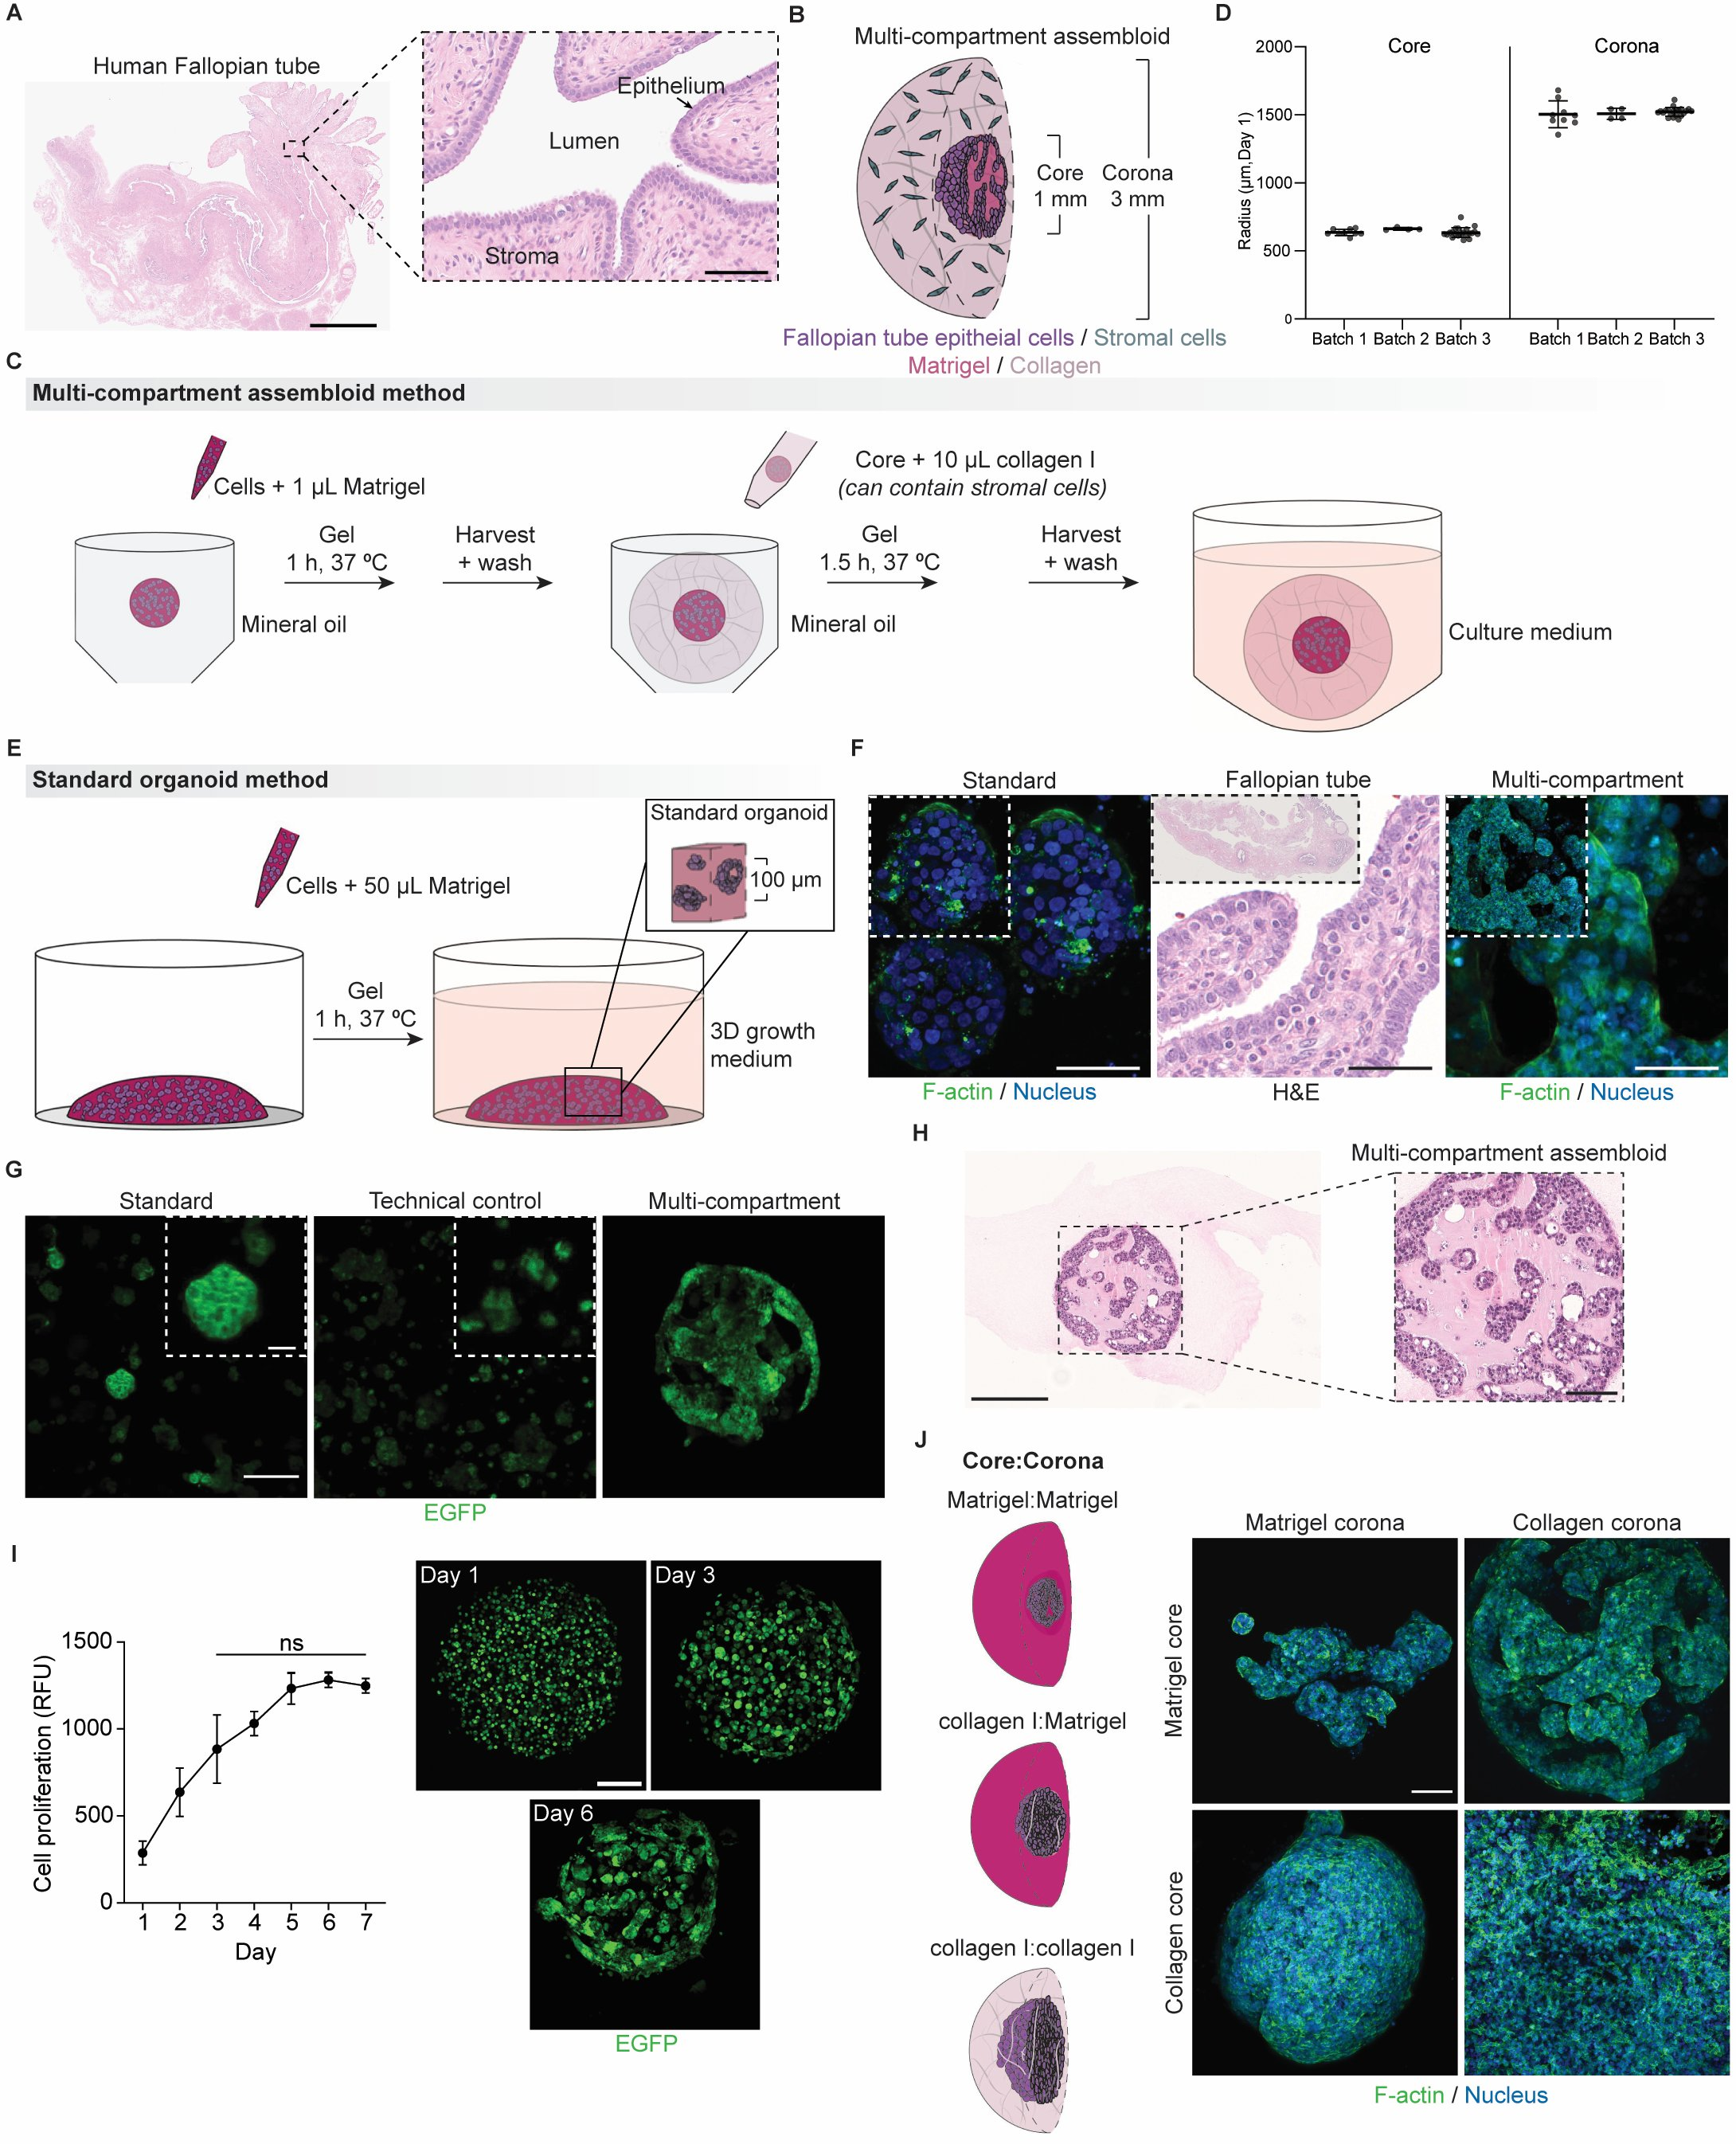
\includegraphics[width=1\textwidth,height=0.85\textheight,keepaspectratio,clip,page=1]{figures/chapter4/fig_1.jpg}
            \captionsetup{font=small}
            \caption{\textbf{Human fallopian tube assembloids.} (A) A healthy human fallopian tube tissue section. Hematoxylin and eosin (H\&E): nuclei (purple), ECM and cytoplasm (pink). Scale bar, 5 mm. Inset, 75 µm. Cartoons depicting (B) a multi-compartment fallopian tube assembloid and (C) the protocol to generate assembloids where stromal cells can be incorporated into the corona (indicated, but not shown). }
            \label{chapter4_fig1}
        \end{center}
    \end{figure}
    
    \begin{figure}[h!]
        \ContinuedFloat
        \captionsetup{font=small}
        \caption[]{(D) The radius of fallopian tube assembloid cores and whole assembloids (corona) were measured from phase-contrast images taken on day 1 of assembloid culture. The size of assembloid cores and coronas are extremely consistent within and between batches. Data are mean ± SD.  (E) Cartoon depicting the protocol to generate standard organoids and a mature standard fallopian tube organoid. (F) Side-by-side comparison of standard organoids (left), human fallopian tube tissue (middle) and multi-compartment assembloids (right). Inset is a whole organoid, fallopian tube, or assembloid. F-actin (green) and nuclear DNA (blue). Fallopian tube tissue is an H\&E stained tissue section. Scale bars, 50 µm. (G) EGFP-tagged FTECs (green) on day 6 grown in the standard organoid model (left), a technical control (middle), and the multi-compartment assembloid model (right). Scale bar, 250 µm. Inset, 50 µm. (H) H\&E image of a fallopian tube multi-compartment assembloid. Scale bar, 300 µm. Inset is the epithelial region of the assembloid. Inset scale bar, 100 µm. (I) PrestoBlue net proliferation in multi-compartment assembloids with timepoint images of EGFP-tagged multi-compartment assembloids (green). Scale bar, 250 µm. N = 3, n = 4+. Statistical test: one-way ANOVA, ns P > 0.05. Data are mean ± SEM. (J) Representative images of multi-compartment assembloids with all permutations to the assembloid ECM. F-actin (green) and nuclear DNA (blue). Scale bar, 100 µm. All organoid/assembloid images are maximum intensity projections of stacks of confocal microscopy images.}
    \end{figure}

    \begin{figure}[p]
        \begin{center}
            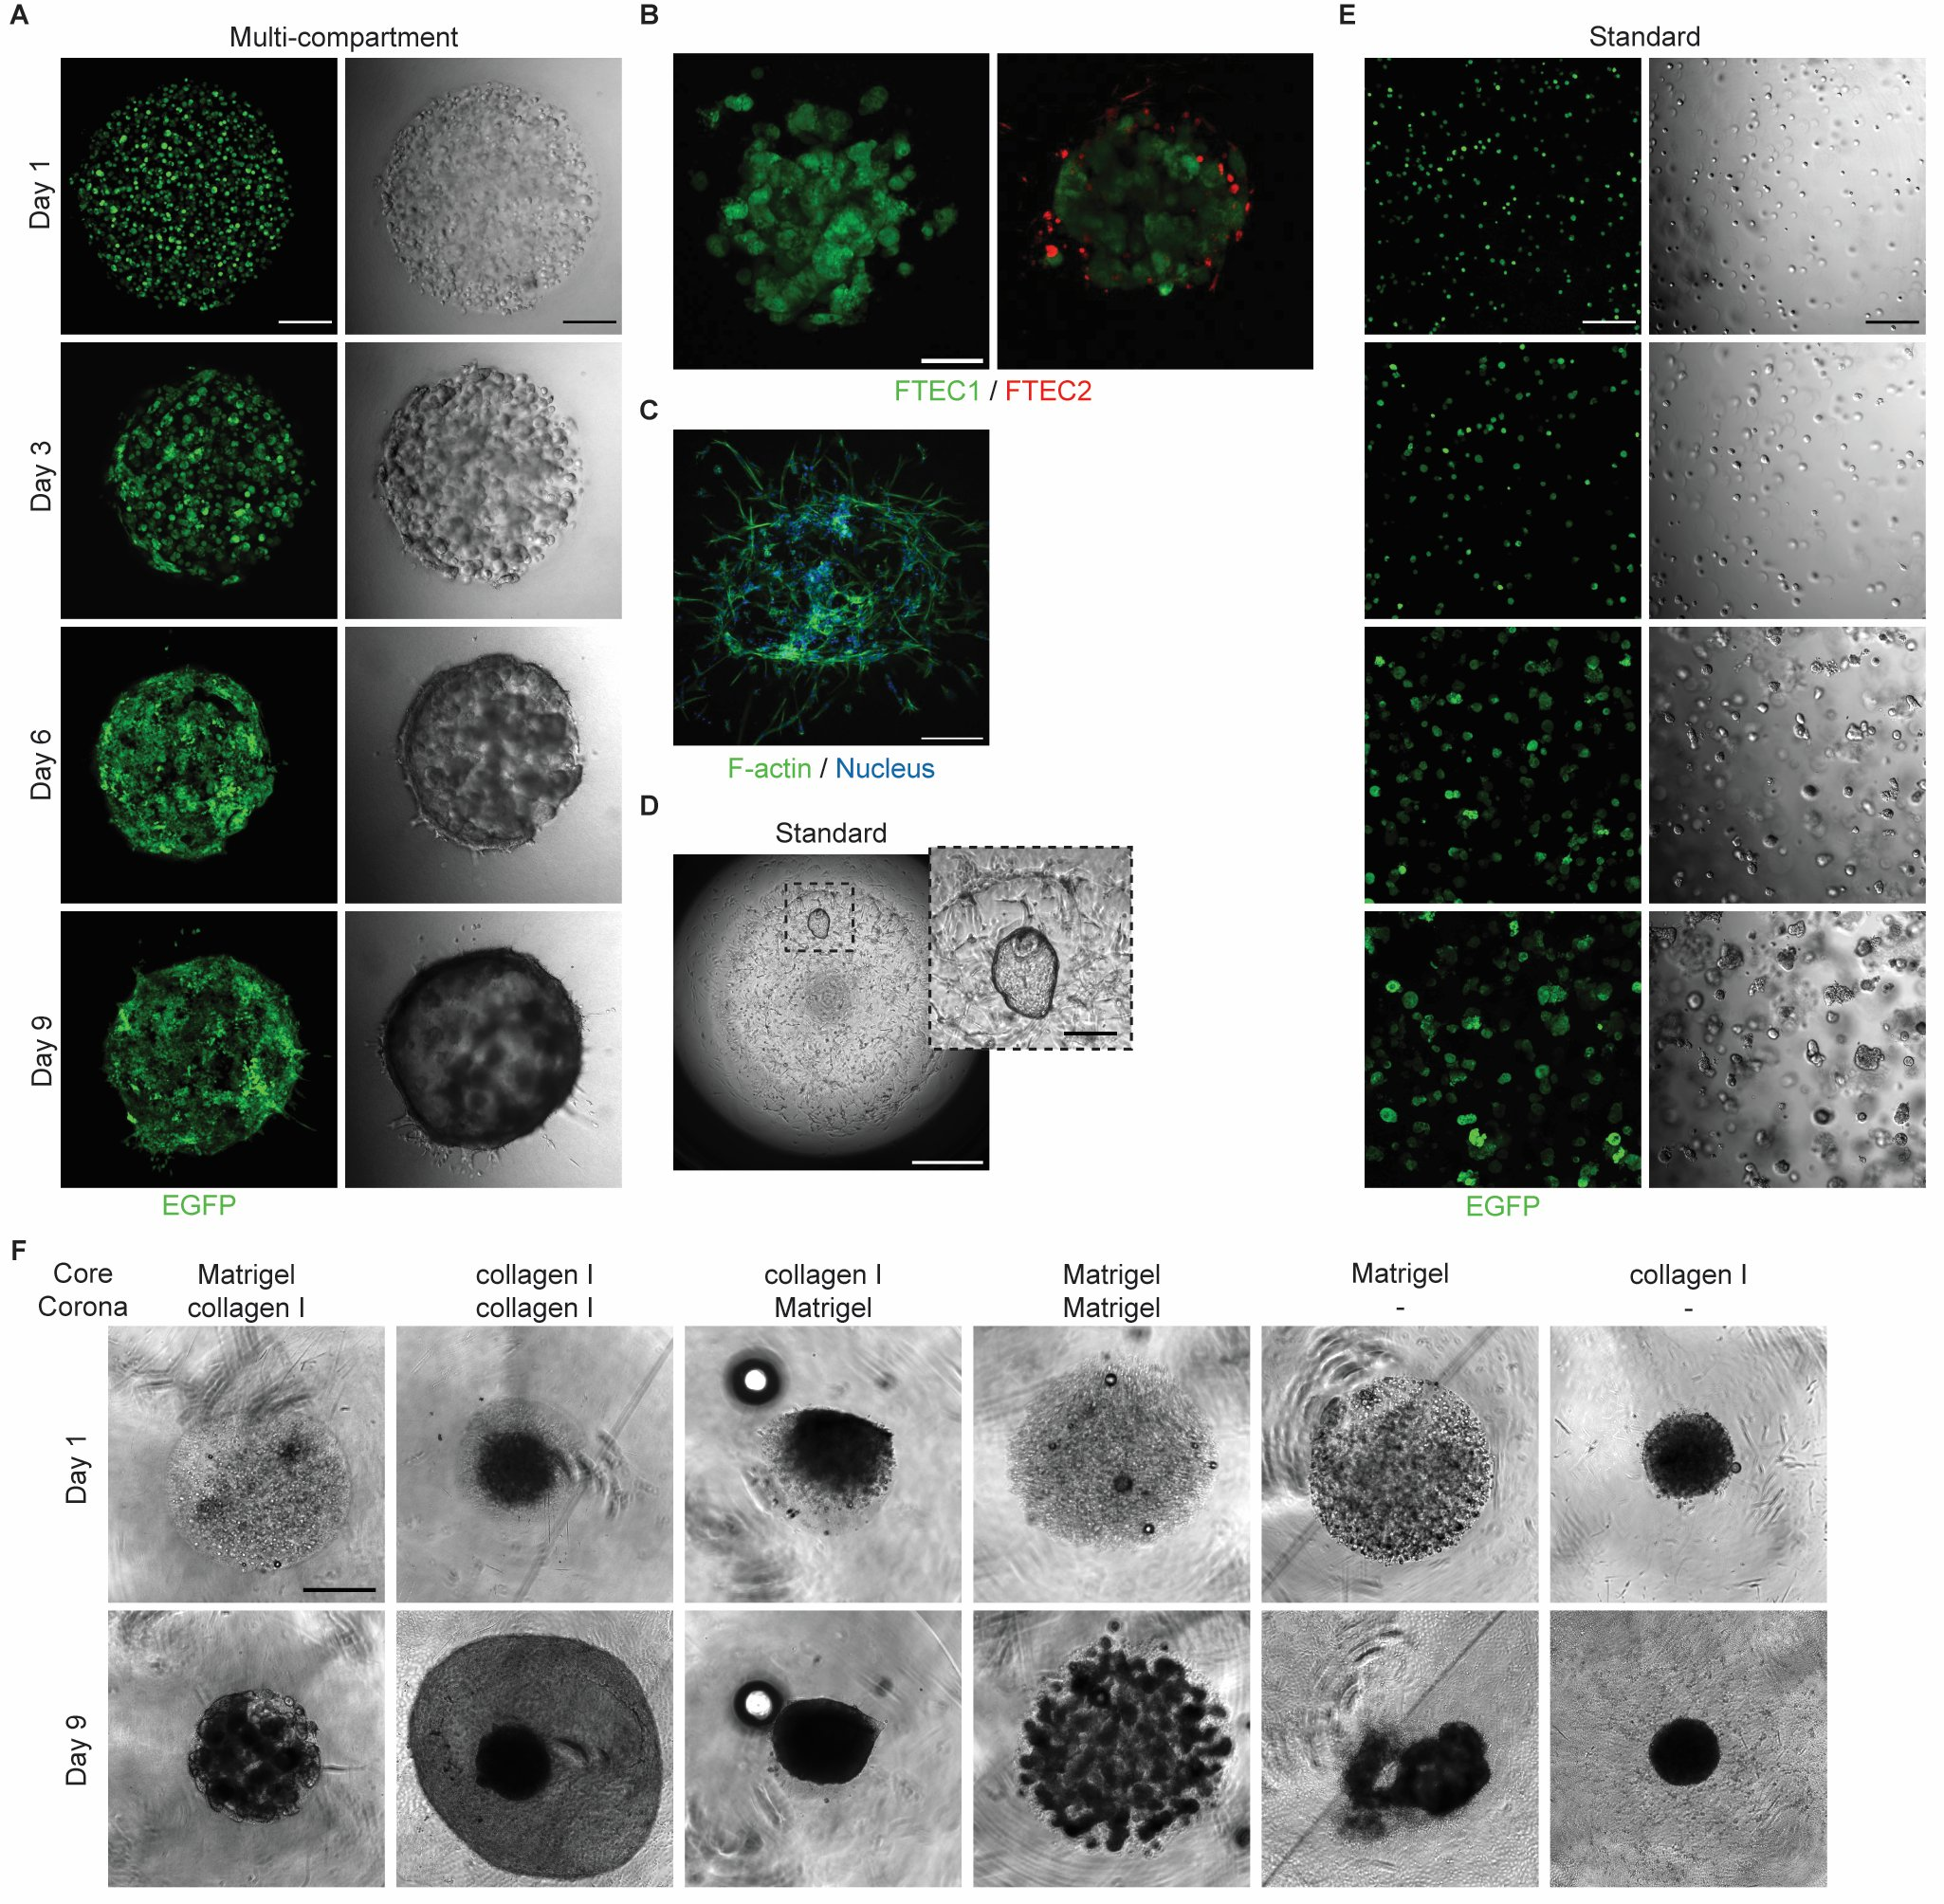
\includegraphics[width=1\textwidth,height=0.85\textheight,keepaspectratio,clip,page=1]{figures/chapter4/fig_S1.jpg}
            \captionsetup{font=small}
            \caption{\textbf{Structural assembly of fallopian tube assembloids.} (A) EGFP-tagged (green) multi-compartment assembloid time series. Images are maximum intensity projections of fluorescence confocal microscopy stacks (left) and DIC (right). Scale bars, 250 µm. (B) Two types of FTECs are mixed in the multi-compartment assembloid core. FTEC cell lines are EGFP (green) and mCherry (red) tagged. Images are maximum intensity projections. Scale bar, 250 µm. (C) Primary FTECs are grown in the multi-compartment assembloid model. Images are maximum intensity projections of fluorescence confocal microscopy stacks. F-actin (green) and nuclear DNA (blue). Scale bar, 250 µm. (D) Primary FTECs are grown in the standard organoid model. Image is phase-contrast microscopy. Scale bar, 1mm. Inset, 250 µm. Inset shows one successfully formed standard organoid. }
            \label{chapter4_figS1}
        \end{center}
    \end{figure}
    
    \begin{figure}[h!]
        \ContinuedFloat
        \captionsetup{font=small}
        \caption[]{  (E) EGFP-tagged (green) standard organoid time series. Images are maximum  intensity projections of fluorescence confocal microscopy stacks (left) and DIC (right). Scale bars, 250 µm. (F) Assembloids with Matrigel or collagen I in the core and all combinations of corona ECM. Phase-contrast images. Scale bar, 500 µm.}
    \end{figure}
    
    \subsection{Multi-compartment assembloids maintain in situ protein expression}
    In addition to the similarity between the fallopian tube’s mucosal folds and the multi-compartment assembloid’s organization, the molecular expression patterns observed in these assembloids also matched the expression patterns observed in a healthy fallopian tube. By direct comparison via immunohistochemistry (IHC) of FFPE tissue sections from a transplantation-quality human fallopian tube (Fig. 2A) and the assembloid (Fig. 1H), we confirmed similar patterns of E-cadherin localization to the lateral cell membranes between epithelial cells (Fig. 2B, fig. S2A). We also confirmed that Ki-67-positive cells were scattered along the assembloid epithelium via immunofluorescence (Fig. 2C, fig. S2B), which matched previously reported patterns in fallopian tube tissues\cite{kessler2015a}. In this healthy fallopian tube assembloid model, MUC16 staining was faint in some clustered regions (Fig. 2D, fig. S2C). An increase in MUC16 expression could be expected in future studies using this model to investigate disease states of the fallopian tube \cite{bast2009a,aithal2018a}, but limited MUC16 staining in this healthy baseline model aligns with physiological expectations. 
    We also confirmed that the multi-compartment assembloid model formed adherens junctions (E-cadherin)\cite{stockinger2001a,soler1999a,bajpai2008a} and tight junctions (occludin)\cite{cummins2012a}, via western blot (fig. S2D). Similar global protein expression was observed in the standard organoid model. Compared to FTECs grown in 2D culture, E-cadherin expression was increased in both 3D models. 
    Beyond these select fallopian tube epithelial markers, label-free data-independent acquisition-mass spectrometry-based proteomics (DIA-MS)\cite{gillet2012a,collins2017a,bons2023a,meier2020a} was performed for a more comprehensive evaluation of the 3D models (fig. S2E). DIA-MS provided reproducible and accurate quantification of the subcellular proteomes (Data S1-S7)\cite{burton2022a,thul1979a} and the matrisomes\cite{bons2023a}, which we further compared to the fallopian tube matrisome previously reported in the Matrisome database\cite{shao2023a}. This analysis was performed on immortalized FTECs (fig. S2F) and primary FTECs (fig. S2G) assembloids to analyze the behavior of FTECs from two different sources in the multi-compartment model. Standard organoids are most often grown from primary FTEC cell cultures\cite{kessler2015a,clevers2016a}, so our primary FTEC multi-compartment assembloids were also compared to primary FTEC standard organoids (fig. S2H). When primary FTECs were cultured in the multi-compartment assembloid model, the total number of quantifiable protein groups with at least two unique peptides was 2,255, which was more than three times the total number of protein groups quantified when the same primary FTECs were cultured in standard organoids with 674 proteins identified (Fig. 2E). An important distinction between the multi-compartment assembloid and standard organoid proteomes is the percentage of protein groups that match with extracellular components: 43\% for FTEC cell line multi-compartment assembloids, 54\% for primary FTEC multi-compartment assembloids, and 77\% for standard organoids (fig. S2I). However, the total number of matrisome proteins identified in multi-compartment assembloids was more than double the number of matrisome proteins identified in standard organoids\cite{shao2023a} (Fig. 2F). 
    Multi-compartment assembloids also expressed more fallopian tube-specific matrisome proteins than standard organoids. This is an important feature of the multi-compartment assembloid because our previous structural analysis revealed that physiological cell-ECM interactions are necessary for mucosal folding organization (Fig. 1J). The multi-compartment assembloids in this study contain Matrigel (GFR, core) and collagen (2 – 6 mg/mL, corona), while standard organoids contain Matrigel (GFR) only. The identified matrisome proteins for all models were in excess of ECM controls (fig. S2J), thus these additional matrisome proteins were produced by cells as the cultures matured, and the increase in matrisome proteins expressed in multi-compartment assembloids was not an artifact of the additional ECM introduced in the model design.
    This comprehensive and quantitative DIA-MS approach on the timsTOF HT mass spectrometer (Bruker) referred to as diaPASEF (parallel accumulation-serial fragmentation combined with data-independent acquisition)\cite{meier2020a} also revealed protein groups in all models (FTEC cell line multi-compartment, primary FTEC multi-compartment, and primary FTEC standard) that are associated with ciliated and secretory Gene Ontology\cite{ashburner2000a,aleksander2023a} cellular components (fig. S2I). These proteins are important for the system’s functional accuracy which we describe in greater detail in the next sections. 

    \begin{figure}[p]
        \begin{center}
            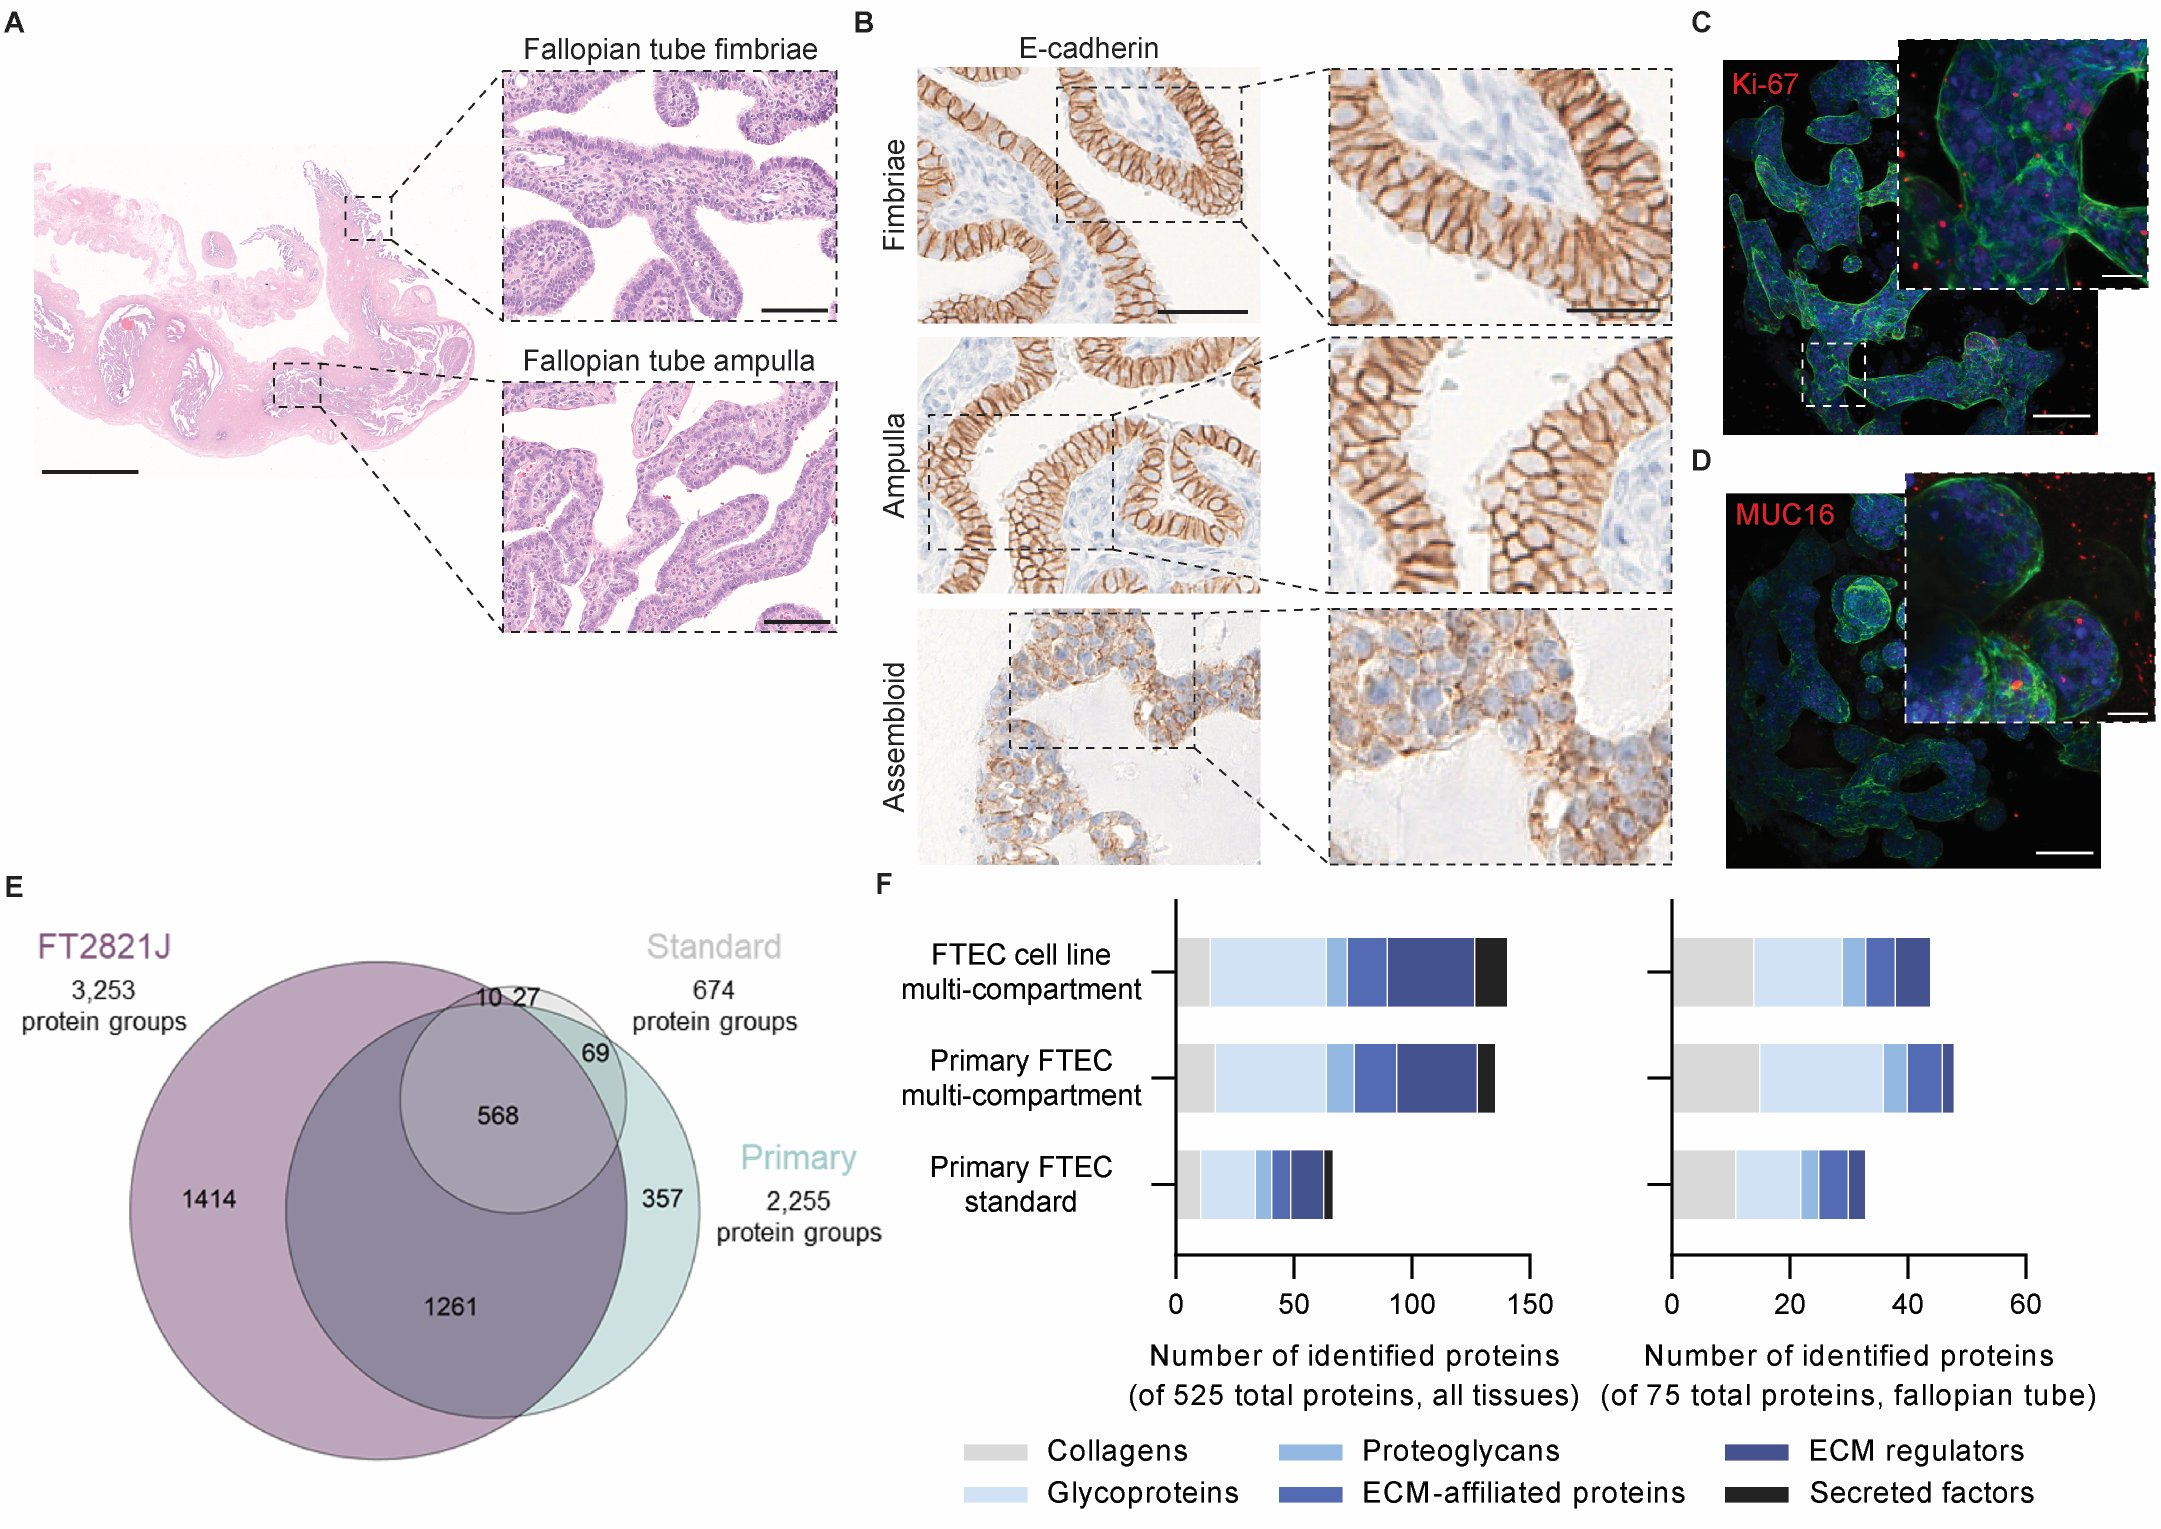
\includegraphics[width=1\textwidth,height=0.85\textheight,keepaspectratio,clip,page=1]{figures/chapter4/fig_2.jpg}
            \captionsetup{font=small}
            \caption{\textbf{Fallopian tube assembloids maintain tissue expression patterns.} (A) H\&E image of a fallopian tube tissue section. Nuclei (purple), ECM and cytoplasm (pink). Scale bar, 5 mm. Top inset is the fallopian tube fimbriae and bottom inset is the fallopian tube ampulla. Inset scale bars, 100 µm. (B) E-cadherin IHC of FFPE tissue sections of the fallopian tube fimbriae (top), fallopian tube ampulla (middle) and fallopian tube assembloid (bottom). Scale bar, 50 µm. Inset, 25 µm. Immunofluorescence staining for (C) Ki-67, and (D) MUC16 in multi-compartment fallopian tube assembloids. Images of assembloids are maximum intensity projections of stacks of confocal microscopy images. Scale bars, 100 µm. Inset scale bars, 20 µm. F-actin (green), nuclear DNA (blue), and protein of interest (red). (E) Venn diagram performed on all quantifiable protein groups (with ≥ 2 unique peptides) in FTEC cell line (purple) and primary FTEC (green) multi-compartment organoids and standard (light grey) organoids. (F) Some proteins identified in the proteomes are categorized in the human matrisome (50) for all tissues (left) and fallopian tube specific (right). (E)-(F) N = 4.}
            \label{chapter4_fig2}
        \end{center}
    \end{figure}

    \begin{figure}[p]
        \begin{center}
            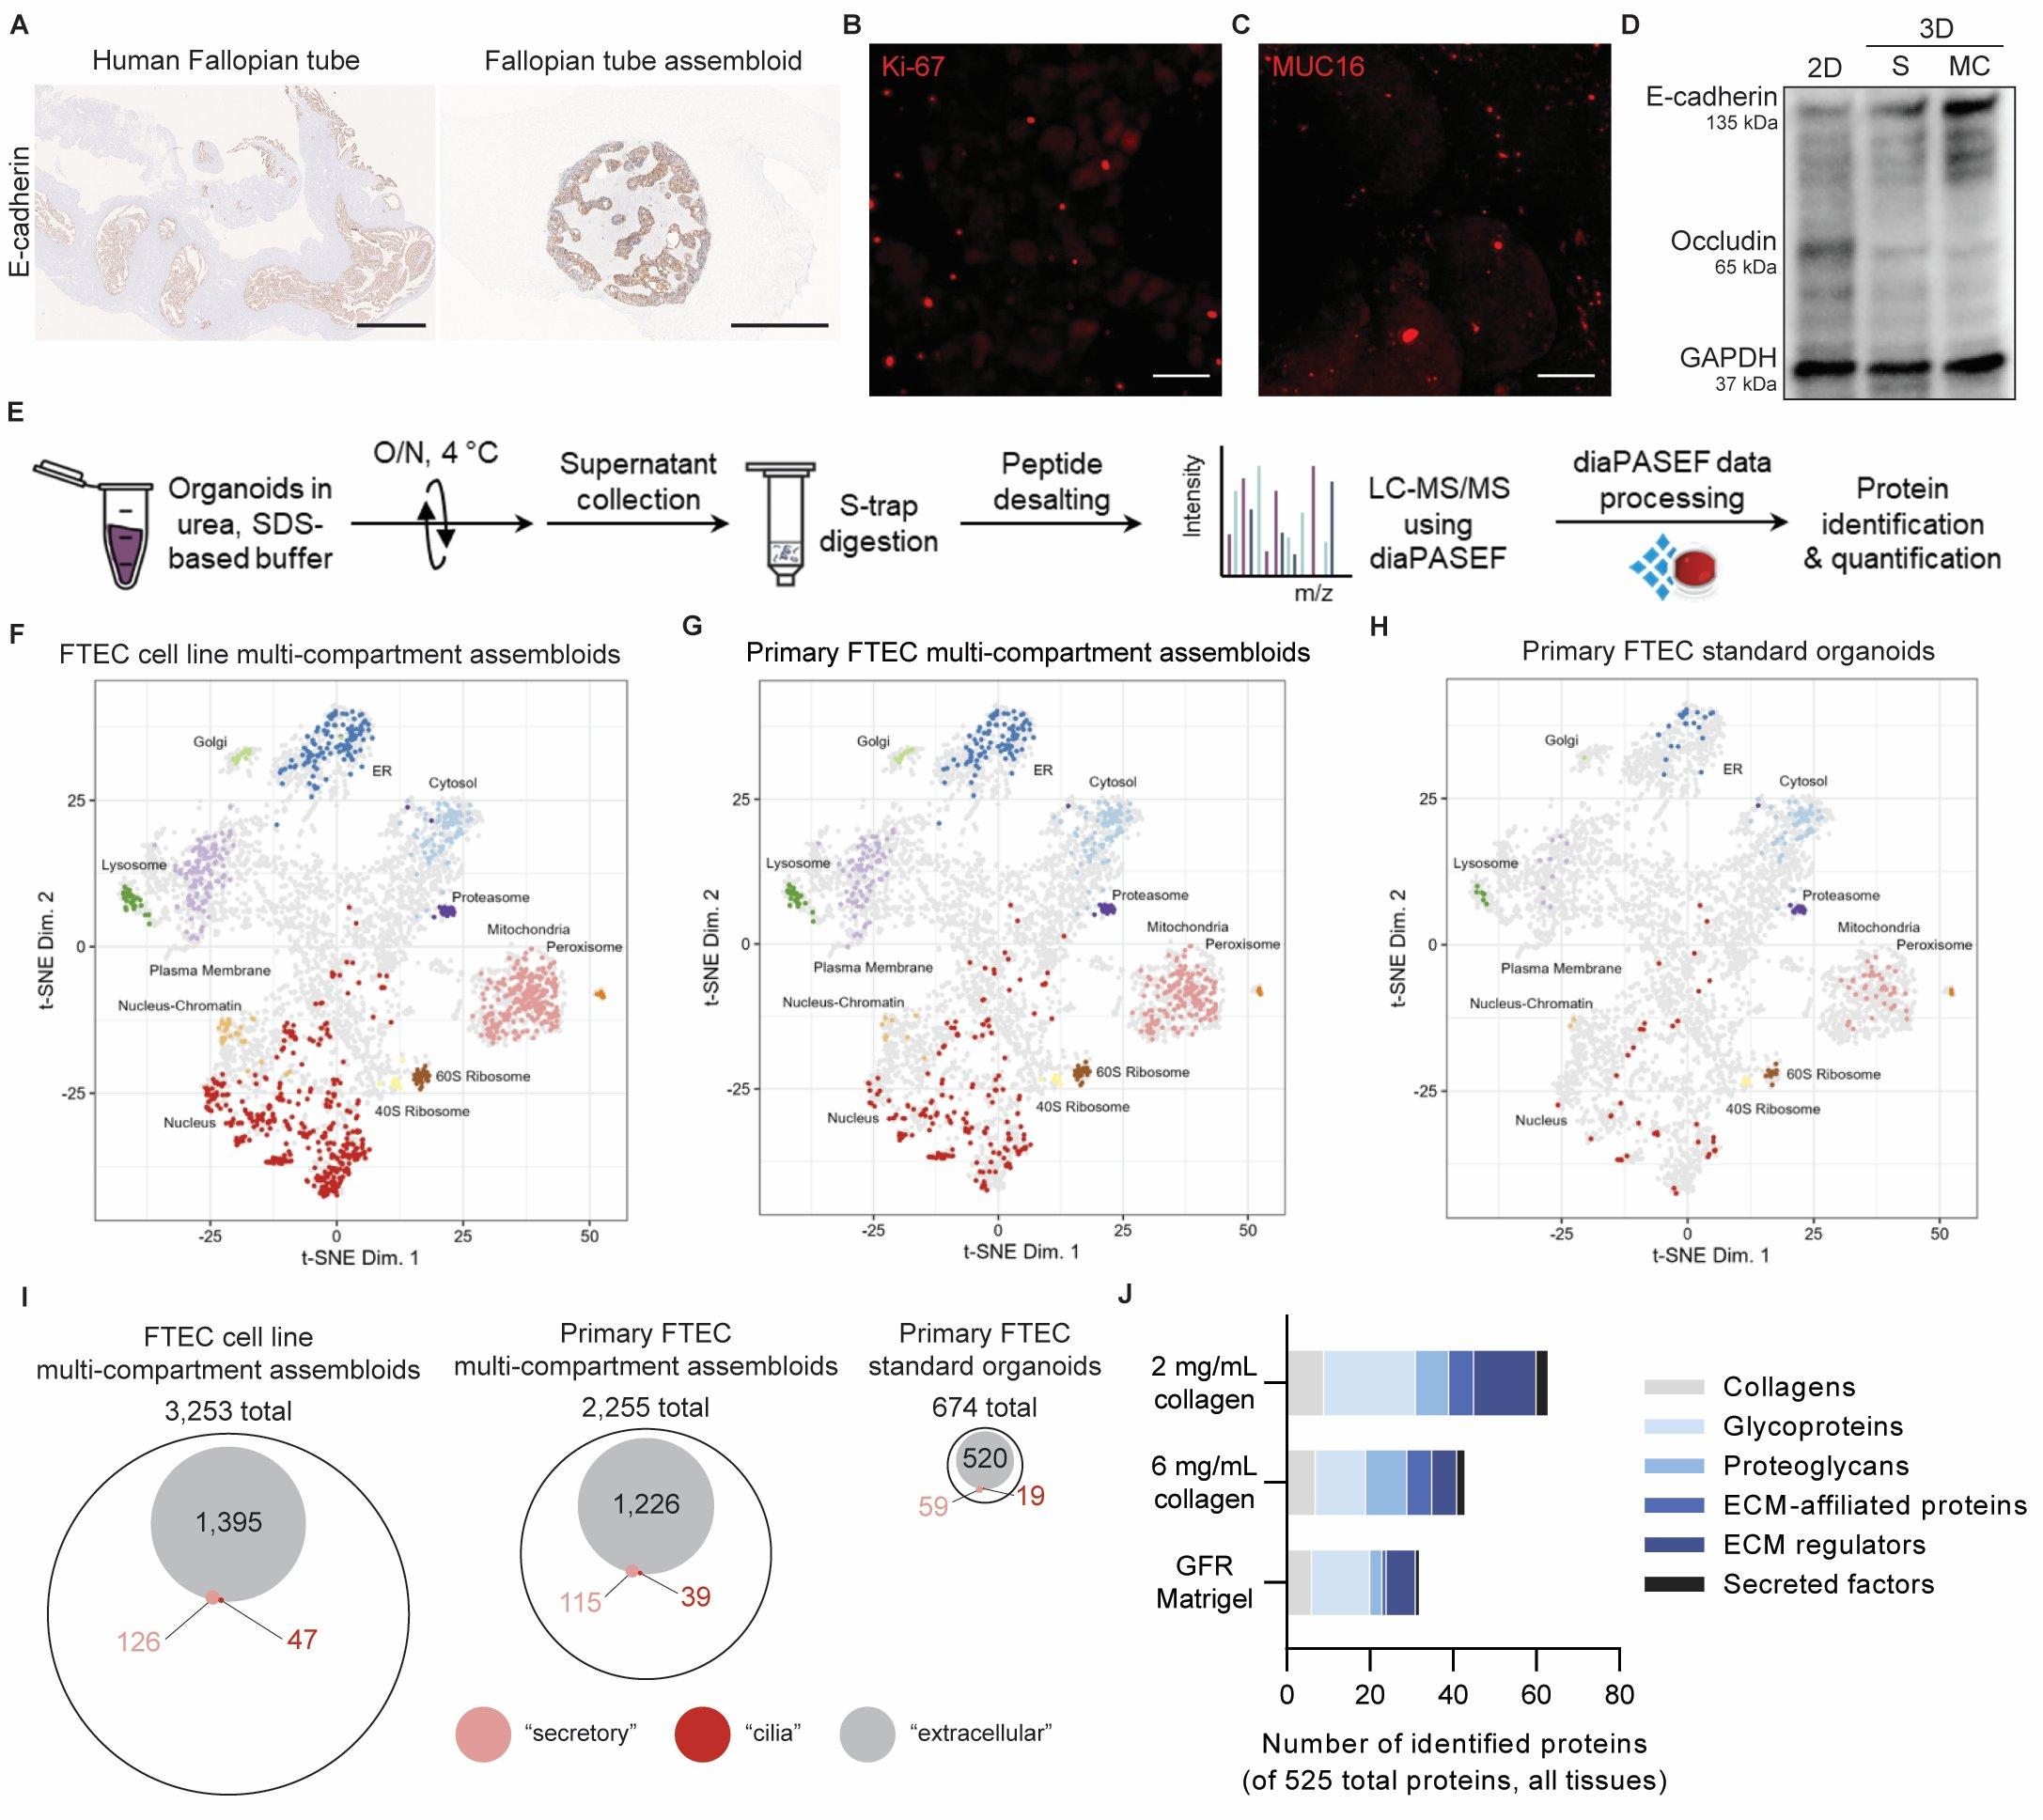
\includegraphics[width=1\textwidth,height=0.85\textheight,keepaspectratio,clip,page=1]{figures/chapter4/fig_S2.jpg}
            \captionsetup{font=small}
            \caption{\textbf{Molecular expression patterns of multi-compartment assembloids and standard organoids.}(A) FFPE tissue sections IHC stained for E-cadherin. Whole, healthy transplantation-quality tissue sections of the fallopian tube (left) and the multi-compartment assembloid (right). Scale bars, 4 mm (left) and 300 µm (right). Isolated protein of interest channel for immunofluorescence images staining (B) Ki-67, and (C) MUC16 in multi-compartment fallopian tube assembloids. Images are maximum intensity projections. Scale bars, 20 µm. (D) Global protein expression in 2D and 3D (S = standard, MC = multi-compartment) culture via western blot. GAPDH is included as a loading control.  (E) Organoids were lysed in a urea SDS-based buffer overnight. Supernants containing solubilized proteins were collected and submitted to trypsin digestion using S-trap. After desalting, proteolytic peptides were analyzed on a timsTOF HT (Bruker) mass spectrometer in diaPASEF mode, and collected MS data were processed using library-free directDIA (Biognosys) for identification and quantification. Subcellular localization of (F) FTEC cell line multi-compartment assembloid, }
            \label{chapter4_figS2}
        \end{center}
    \end{figure}
    
    \begin{figure}[h!]
        \ContinuedFloat
        \captionsetup{font=small}
        \caption[]{ (G) primary FTEC multi-compartment assembloid, and (H) primary FTEC standard organoid proteins via LOPIT map (48, 49, 54, 55). (I) Total protein groups with at least two unique peptides in FTEC cell line multi-compartment assembloids (left), primary FTEC multi-compartment assembloids (middle) and primary FTEC standard organoids (right), and the protein groups with secretory (pink), cilia (red) and extracellular (gray) Gene Ontology (52, 53) cellular components. (J) Proteins identified in the ECM control proteome are categorized in the human matrisome (50) for all tissues. (F)-(J) N = 4.}
    \end{figure}
    
    \subsection{Epithelial differentiation can be stimulated in multi-compartment assembloids}
    The fallopian tube epithelium is composed of a mixture of ciliated and secretory epithelial cells, which have key roles in oocyte transport and survival, respectively\cite{yuan2021a,suarez2021a,wanggren2008a}. IHC analysis of healthy fallopian tube tissue revealed a mixture of PAX8-positive (secretory) and PAX8-negative (ciliated)\cite{kessler2015a,perets2013a,chaves-moreira2022a,karst2011a,karst2012a} epithelial cells (Fig. 3A, fig. S3A). However, most FTECs in the assembloid were PAX8-positive. By transmission electron microscopy (TEM), we identified secretory epithelial cells and cells with cilia or microvilli facing the Matrigel region of the assembloid (Fig. 3B), resembling the lumen of the fallopian tube\cite{kessler2015a}. Tight junctions formed between epithelial cells at the assembloid-Matrigel (lumen-like) and assembloid-collagen I (stroma-like) interfaces, but epithelial secretions and cilia or microvilli were only found at the Matrigel interface (lumen-like) (Fig. 3B,C), matching the tissue anatomy. By contrast, standard organoids also formed tight junctions and showed both cilia and secretions (fig. S3B); however, in standard organoids, cilia or microvilli could be found at multiple locations on both the organoid interior (lumen-like) and exterior (stroma-like) interfaces. 
    While IHC demonstrated that most of the FTECs in the assembloid were secretory, TEM revealed that some assembloid epithelial cells could become ciliated. Secretory FTECs can differentiate into ciliated FTECs upon hormone stimulation\cite{fitzgerald2019a,donnez1985a,comer1998a,comer1998a,garcia-alonso2021a}, so we treated our assembloids with \textbeta-estradiol (E2) and progesterone (P4), two steroid hormones of the menstrual cycle that elicit morphological and functional responses from the fallopian tube epithelium (67). The resulting molecular response was measured via RT-qPCR (Fig. 3D). We observed overall increases in estrogen receptor 1 (ESR1) expression with \textbeta-estradiol treatment and a slight increase with progesterone treatment, matching previously reported responses in fallopian tube tissue\cite{brodowska2021a} and mouse FTEC standard organoids\cite{xie2018a}. In the follicular phase when estrogen is high and progesterone is low \cite{monis-a}, progesterone receptor levels increase in the fallopian tube epithelium\cite{akison2012a} and, accordingly, progesterone receptor (PGR) expression increased when our assembloids were treated with \textbeta-estradiol. \textbeta-estradiol treatment also caused a decrease in the relative expression of secretory cell marker PAX8, which is evidence of ciliated FTEC differentiation (Fig. 3E). The relative expression of markers related to cilia motility/regulatory transcription factor (FOXJ1)\cite{yu2008a,turco2017a} and stem cell differentiation into ciliated cells (OLFM4)\cite{gu2020a,li2020a} also increased with \textbeta-estradiol stimulation. The relative expression of MKI67 was not significantly changed from the untreated control (Fig. 3F), which aligns with previous reports of null or limited proliferation of oviductal epithelium when stimulated with estradiol\cite{eddie2015a,moyle-heyrman2016a}. Standard organoids did not always produce these expected responses to hormone treatment (fig. S3C). The relative expression of MKI67 was significantly reduced when treated with progesterone, and markers of morphological cell type (PAX8, FOXJ1) were unchanged from controls with \textbeta-estradiol stimulation (fig. S3D). Progesterone also prompted an unexpected increase in TNF expression. These results demonstrated a physiological response to steroid hormone stimulation by the healthy fallopian tube assembloid, and that the ratio of ciliated:secretory epithelial cells in multi-compartment assembloids can be tuned to better match the composition of the tissue epithelium.
    While cilia and smooth muscle are both involved in the transport of an oocyte through the fallopian tube, motile cilia are especially important when capturing and initiating oocyte transport in the infundibulum region near the ovary\cite{yuan2021a,suarez2021a,wanggren2008a}. Cilia are vital to a functional fallopian tube, and thus, cilia must be present in an assembloid aiming to capture the physiological fallopian tube. As an additional confirmation of ciliation potential, we identified Gene Ontology\cite{ashburner2000a,Ashburner2000Gene} biological processes that were upregulated when multi-compartment assembloids were treated with \textbeta-estradiol via diaPASEF-MS-based proteomics\cite{meier2020a} and ConsensusPathDB\cite{kamburov2011a,kamburov2011a} (Fig. 3G-I). This analysis was performed on cell line (Fig. 3G) and primary (Fig. 3H) multi-compartment assembloids to demonstrate the functional capacity of the assembloid model with cells from multiple sources. For each condition, the average coefficient of variation (CV) across biological replicates in the proteomics dataset ranged between 20\% and 39\% at the protein level (fig. S3E), demonstrating good reproducibility for large-scale discovery and quantitative analytical assays that monitor thousands of proteins. HSPG2 was among the protein groups upregulated in both primary and cell line assembloids stimulated with \textbeta-estradiol, which has been linked to reproductive functions including tissue development and blastula implantation\cite{chen2023a,garcia2024a}.  \textbeta-estradiol stimulation also resulted in upregulation of cytoskeleton-related biological processes including cytoskeleton organization and epithelial cell differentiation (FT2821J cell line) and plasma membrane bounded cell projection organization and cell motility/migration (primary) (Fig. 3I). Among other processes regarding epithelial cell junction and ECM/basement membrane assembly, these upregulated biological processes confirm assembloid epithelial maturation upon \textbeta-estradiol stimulation, including the differentiation of secretory cells into ciliated cells and cilia motility\cite{park2008a,antoniades2014a,garcia2018a}.

    \begin{figure}[p]
        \begin{center}
            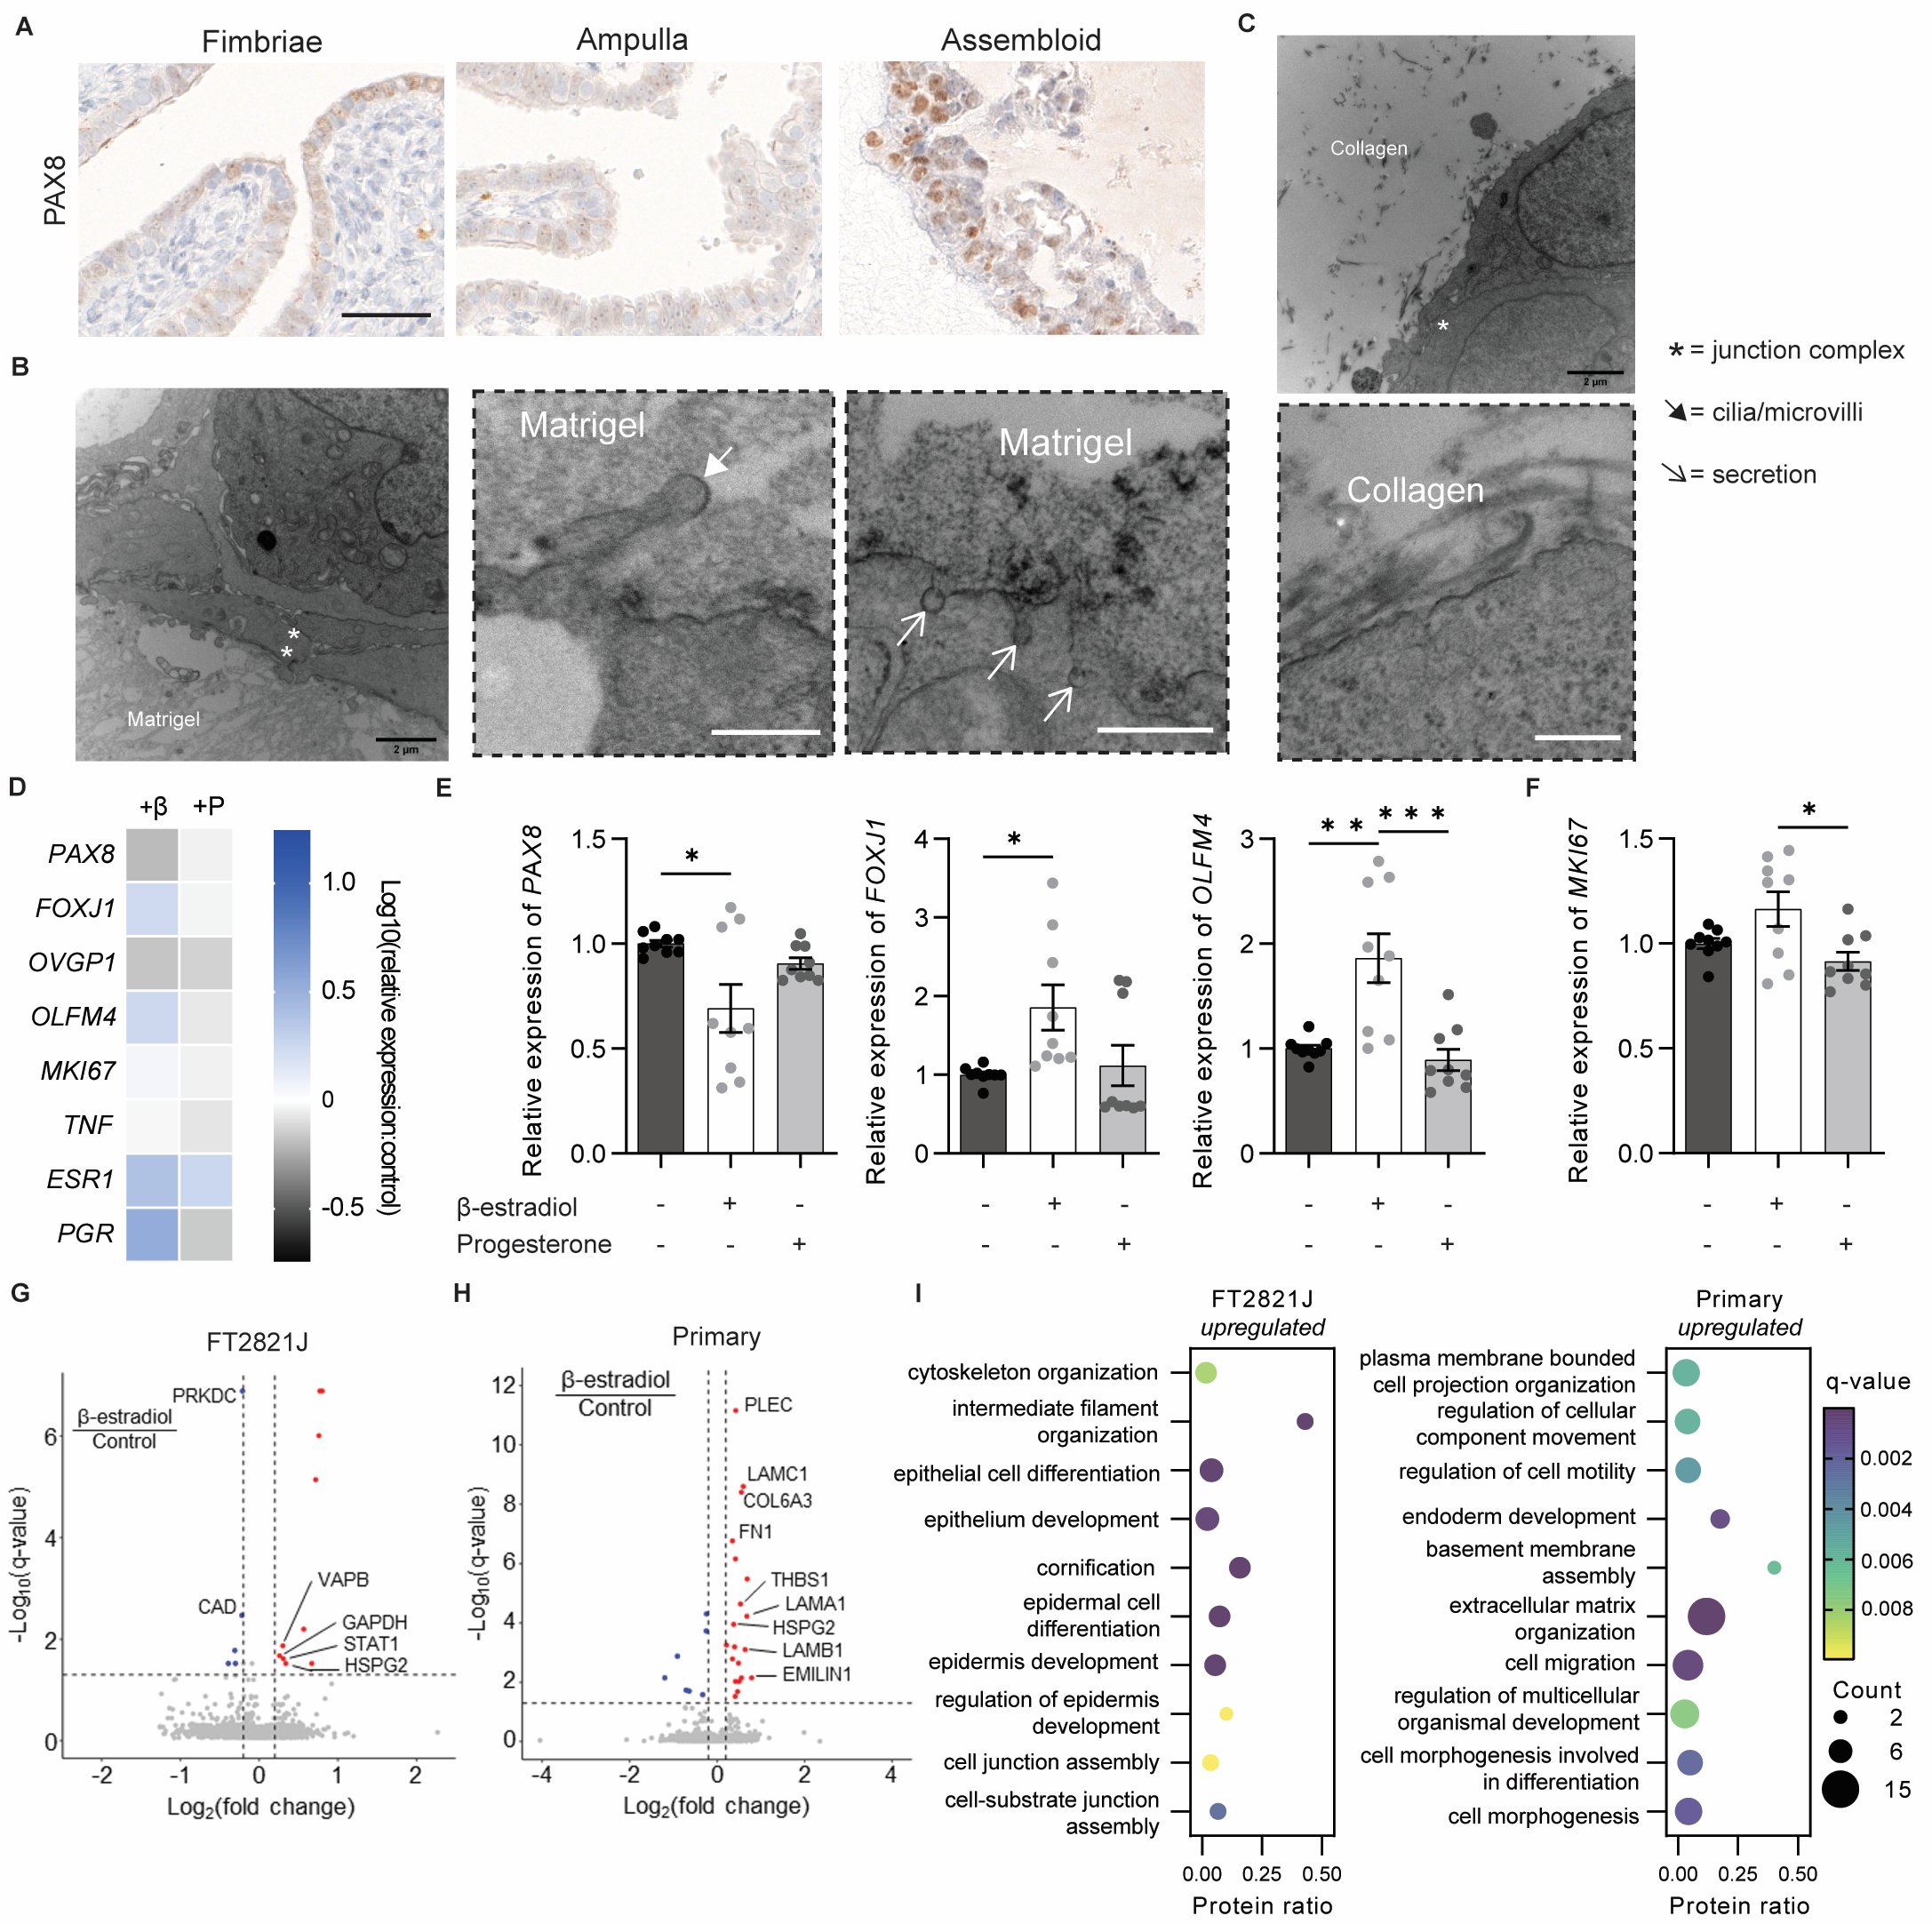
\includegraphics[width=1\textwidth,height=0.85\textheight,keepaspectratio,clip,page=1]{figures/chapter4/fig_3.jpg}
            \captionsetup{font=small}
            \caption{\textbf{Epithelial composition of multi-compartment assembloids.} (A) PAX8 IHC of FFPE tissue sections of the fallopian tube fimbriae (top), fallopian tube ampulla (middle) and fallopian tube assembloid (bottom). Scale bar, 50 µm.  TEM of the (B) cell-Matrigel (lumen-like) interface and (C) cell-collagen I (stroma-like) interface of a multi-compartment assembloid. Scale bars, 2 µm. Inset scale bars, (B) 500 nm (both) and (C) 300 nm. Asterisk = junction complex, filled arrow = cilia/microvilli, open arrow = secretion. (D) RT-qPCR of β-estradiol (β) or progesterone (P) treated multi-compartment assembloids. Data are log10(relative expression:untreated control). Relative expression of genes related to (E) ciliated differentiation and (F) proliferation. }
            \label{chapter4_fig3}
        \end{center}
    \end{figure}
    
    \begin{figure}[h!]
        \ContinuedFloat
        \captionsetup{font=small}
        \caption[]{(D)-(F) N = 3, n = 3. Statistical tests: one-way ANOVA with multiple comparisons, ***P $≤$ 0.001, **P $≤$ 0.01, *P ≤ 0.05. All data are mean $±$ SEM. Volcano plot of upregulated (red)/downregulated (blue) protein groups when (G) FTEC cell line multi-compartment assembloids and (H) primary FTEC multi-compartment assembloids were treated with \textbeta-estradiol (statistical significance: q-value $≤$ 0.05 and absolute log2(fold-change) $≥$ 0.2). (I) Gene Ontology\cite{Ashburner2000Gene, ashburner2000a} biological processes that were upregulated in \textbeta-estradiol treated FTEC cell line (left) and primary FTEC (right) multi-compartment assembloids. Relative protein quantification assessed by DIA-MS (47) and subsequent enrichment analysis performed using ConsensusPathDB\cite{kamburov2009a,kamburov2011a}. N = 4.}
    \end{figure}

    \begin{figure}[p]
        \begin{center}
            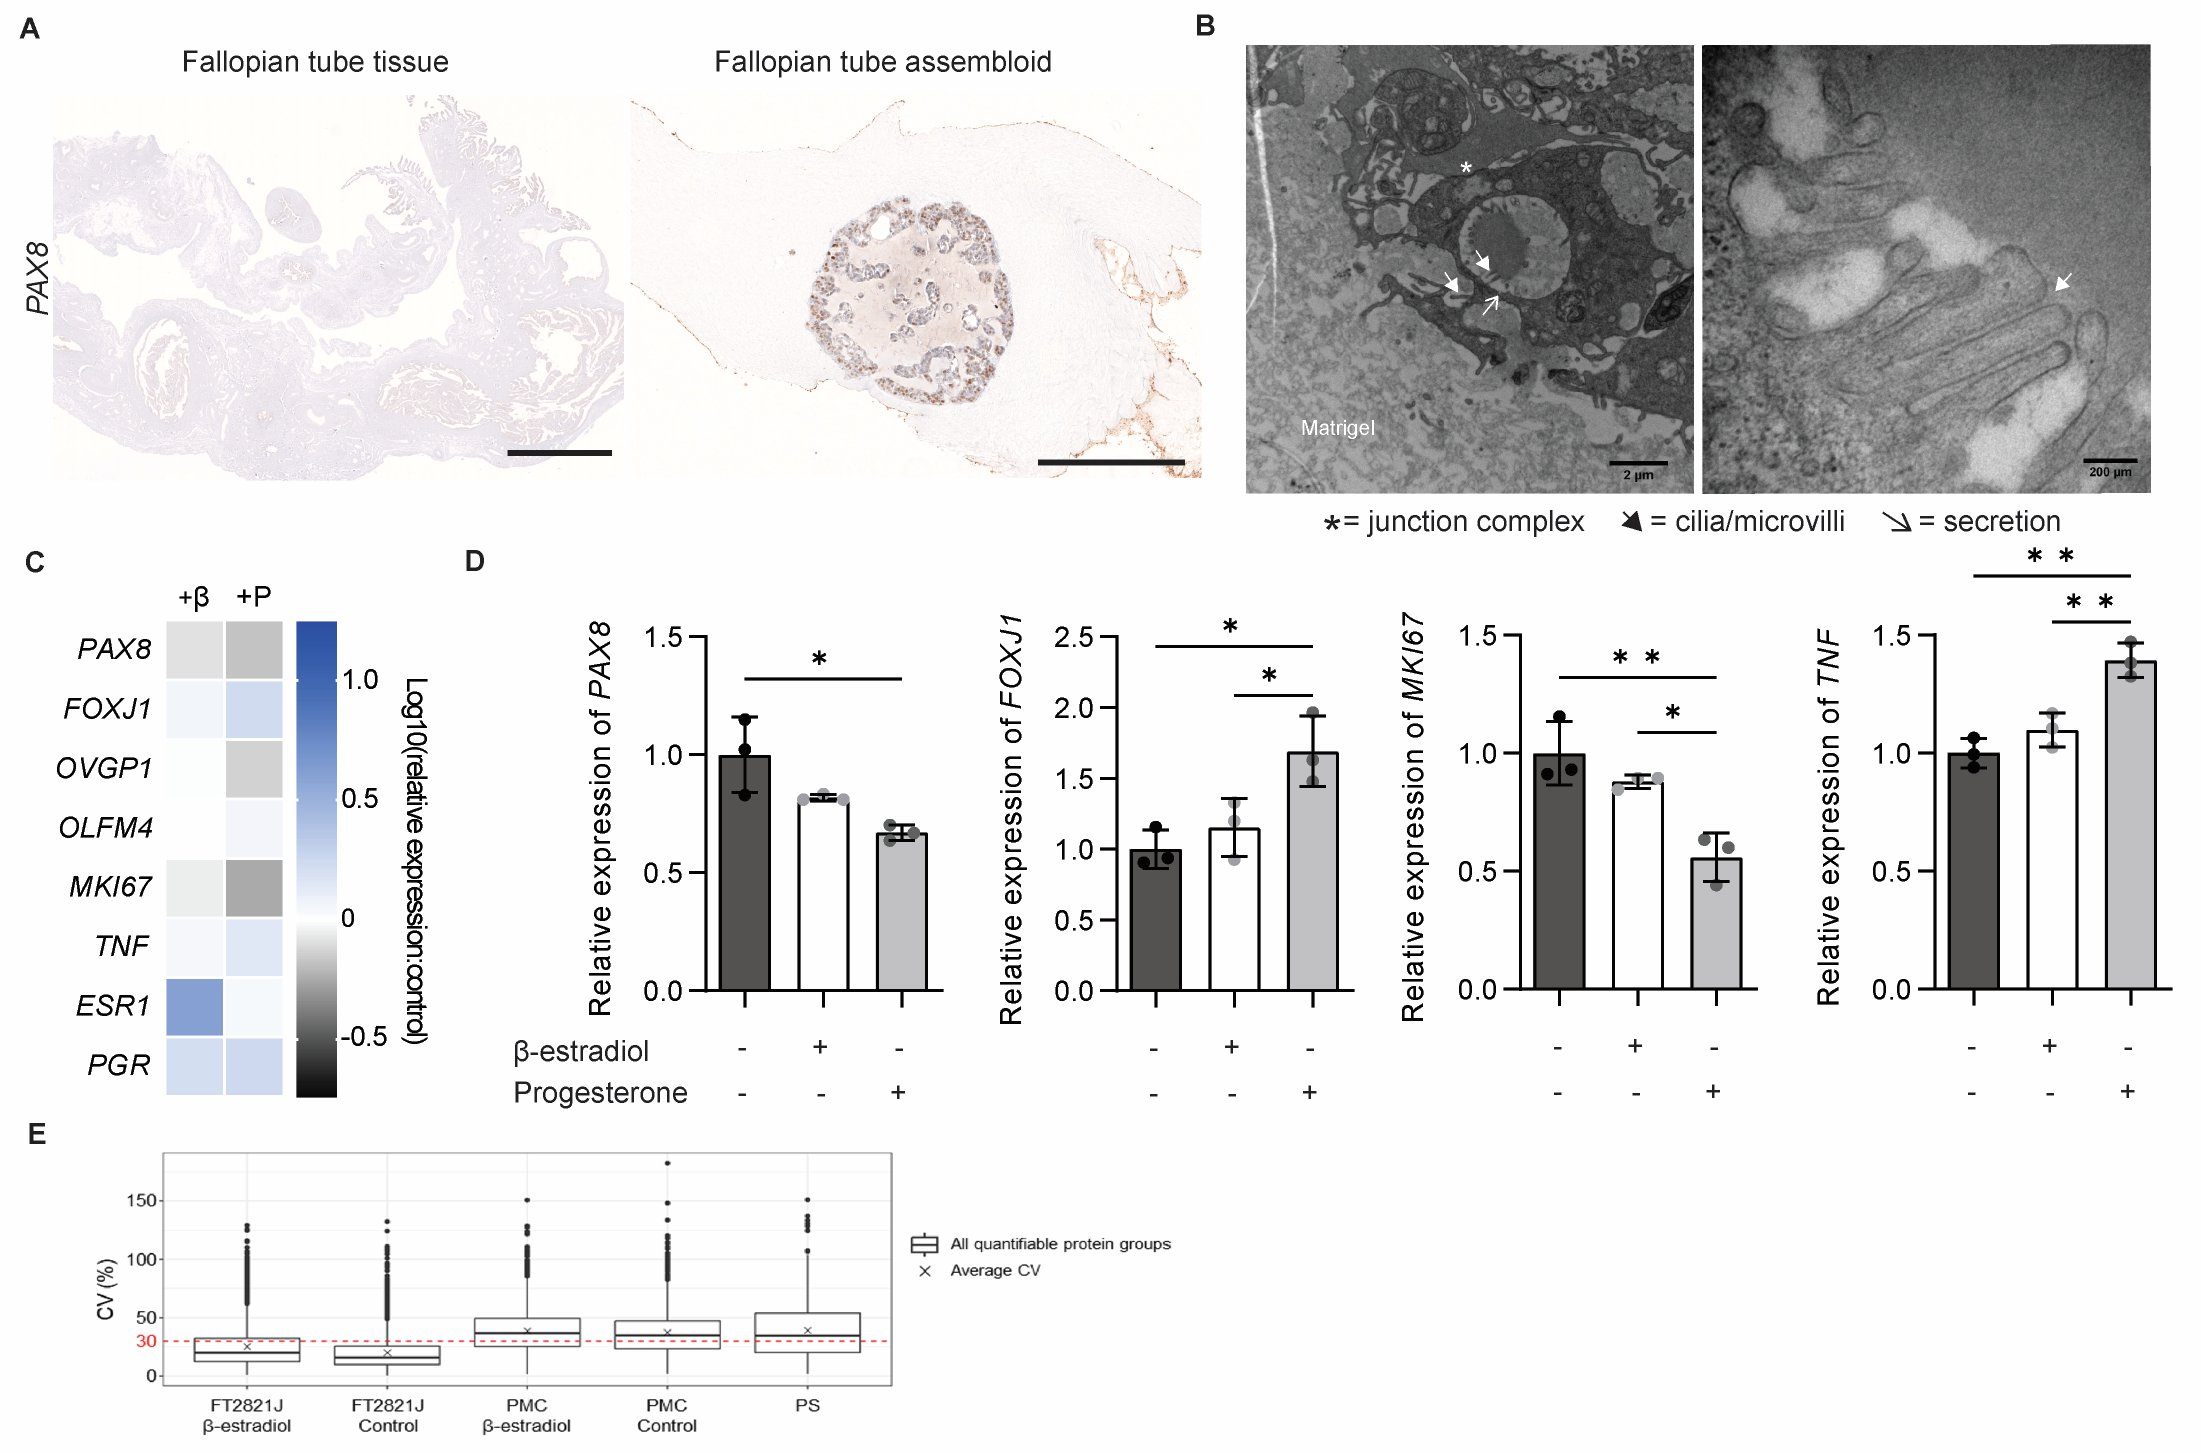
\includegraphics[width=1\textwidth,height=0.85\textheight,keepaspectratio,clip,page=1]{figures/chapter4/fig_S3.jpg}
            \captionsetup{font=small}
            \caption{\textbf{Epithelial composition of the fallopian tube in vitro models.} (A) FFPE tissue sections IHC stained for PAX8. Whole, healthy transplantation-quality tissue sections of the fallopian tube (top) and the multi-compartment assembloid (bottom). Scale bars, 4 mm (top) and 300 µm (bottom). (B) Transmission electron microscopy of a standard fallopian tube organoid. Scale bar, 2 µm (left) and 200 nm (right). Asterisk = junction complex, filled arrow = cilia/microvilli, open arrow = secretion. (C) RT-qPCR of β-estradiol (β) or progesterone (P) treated standard organoids. Data are log10(relative expression:untreated control). (D) Relative expression of genes related to cell differentiation into ciliated epithelial cells and proliferation in standard organoids. Data are mean ± SD. Statistical test: one-way ANOVA with multiple comparisons, **P ≤ 0.01, *P ≤ 0.05.  (C)-(D) N = 1, n = 3. (E) Coefficients of variation (CVs) were calculated on the protein group abundance of four replicates. The boxplots display the CV distribution obtained for the FTEC cell line multi-compartment organoids (FT2821J), primary FTEC multi-compartment organoids (PMC) and primary standard organoids (PS), using all quantifiable protein groups (with ≥ 2 unique peptides). Good reproducibility using diaPASEF-MS was achieved among organoid replicates (n = 4), with overall average CVs ranging between 20\% and 39\%, which is compatible with large-scale discovery and quantification assays. N = 4.}
            \label{chapter4_figS3}
        \end{center}
    \end{figure}
    
    % \begin{figure}[h!]
    %     \ContinuedFloat
    %     \captionsetup{font=small}
    %     \caption[]{ (G) primary FTEC multi-compartment assembloid, and (H) primary FTEC standard organoid proteins via LOPIT map (48, 49, 54, 55). (I) Total protein groups with at least two unique peptides in FTEC cell line multi-compartment assembloids (left), primary FTEC multi-compartment assembloids (middle) and primary FTEC standard organoids (right), and the protein groups with secretory (pink), cilia (red) and extracellular (gray) Gene Ontology (52, 53) cellular components. (J) Proteins identified in the ECM control proteome are categorized in the human matrisome (50) for all tissues. (F)-(J) N = 4.}
    % \end{figure}
    
    \subsection{Activated multi-compartment assembloids reproduce the function of the organ}
    From a functional perspective, the differentiation of FTECs into ciliated epithelial cells in response to \textbeta-estradiol stimulation is important. Cilia need to be expressed in the epithelium, and these cilia need to also be motile and able to transport an object (oocyte) along the epithelium\cite{yuan2021a,suarez2021a,wanggren2008a}. To test the function of cilia induced by \textbeta-estradiol treatment and demonstrate the multi-compartment fallopian tube assembloid’s mechanical function, we developed a bead displacement assay where oocyte-mimicking fluorescent microbeads were mixed in the lumen-like region of assembloids (Fig. 4A). Some of these assembloids were stimulated with \textbeta-estradiol to induce ciliated differentiation of their epithelial cells. After 7 days of growth the assembloids had matured, and microbeads transported along the interface of the assembloid epithelium and the lumen-like region were tracked using time-lapse confocal microscopy (Fig. 4B, Video S1). The trajectories of beads were more irregular and covered larger distances when assembloids were treated with \textbeta-estradiol than in untreated controls (Fig. 4C). The stimulated trajectories were much larger than cell movement within the assembloids or the system noise without any cells, and followed the curvature of the assembloid epithelium. This was quantitatively verified by calculating the mean squared displacements (MSDs) of the microbeads over 8h (Fig. 4D) and the microbead velocity (Fig. 4E)\cite{wirtz2009a,wu2015a}. While there was no significant difference in the persistence of microbead movement from the untreated control (persistence time), the total microbead diffusivity was increased in the \textbeta-estradiol treated condition (fig. S4A). 
    The RT-qPCR and DIA-MS proteomics results presented earlier (Fig. 3D-G) indicated an increase in ciliated cells when these assembloids were treated with \textbeta-estradiol. As an additional confirmation that the increase in microbead movement could be due to motile cilia, \textbeta-estradiol treated and untreated assembloids were digested, cells were isolated from assembloid debris, and cell motility in DPBS was tracked (Fig. 4F, Video S2). If cells had motile cilia, the cilia acted as a motor propelling suspended cells through DPBS\cite{garcia2018a} (Fig. 4G). Cells isolated from \textbeta-estradiol treated assembloids had higher MSDs than cells isolated from the untreated assembloids (Fig. 4H). Together, the data collected from \textbeta-estradiol stimulated assembloids via RT-qPCR, DIA-MS proteomics, and the cilia-driven motility assay concluded that the increased microbead movement observed in \textbeta-estradiol stimulated assembloids was the result of functional cilia along the assembloid epithelium-lumen interface. Thus, multi-compartment assembloids capture the organ’s mechanical function.
    The same bead displacement assay was performed in standard organoids (fig. S4B). Individual standard organoids grow from a single parent cell where a lumen forms in the center of an individual organoid\cite{kessler2015a}. Due to the nature of organoid maturation in the standard model, standard organoids either encased microbeads in the organoid lumen-like region or contacted microbeads along the external epithelial surface (fig. S4C). However, our electron microscopy results had previously revealed that standard organoids can form cilia or microvilli on the lumen-like and external epithelial surfaces (fig. S3B), so microbeads in contact with any surface of the organoid could be moved by cilia if the cilia were motile. The trajectories of beads tracked in standard organoids revealed larger trajectories in the untreated organoids than in those treated with \textbeta-estradiol (fig. S4D). The quantification of these trajectories also showed little difference in the microbead velocities of any experimental group (fig. S4E); although, microbead MSDs in untreated organoids were increased compared to the noise of the system (fig. S4F). There was no statistically significant difference in the persistence time or total diffusivity for the microbeads tracked in these experimental groups (fig. S4G). Together, these results suggest that bead movement in standard organoids was more likely due to the movement of cells than motile cilia induced by hormone stimulation.
    These functional assessments demonstrate that the multi-compartment assembloids resemble the fallopian tube organ in both hormone response and transport ability, thus displaying functional similarity to the organ.
    
    \begin{figure}[p]
        \begin{center}
            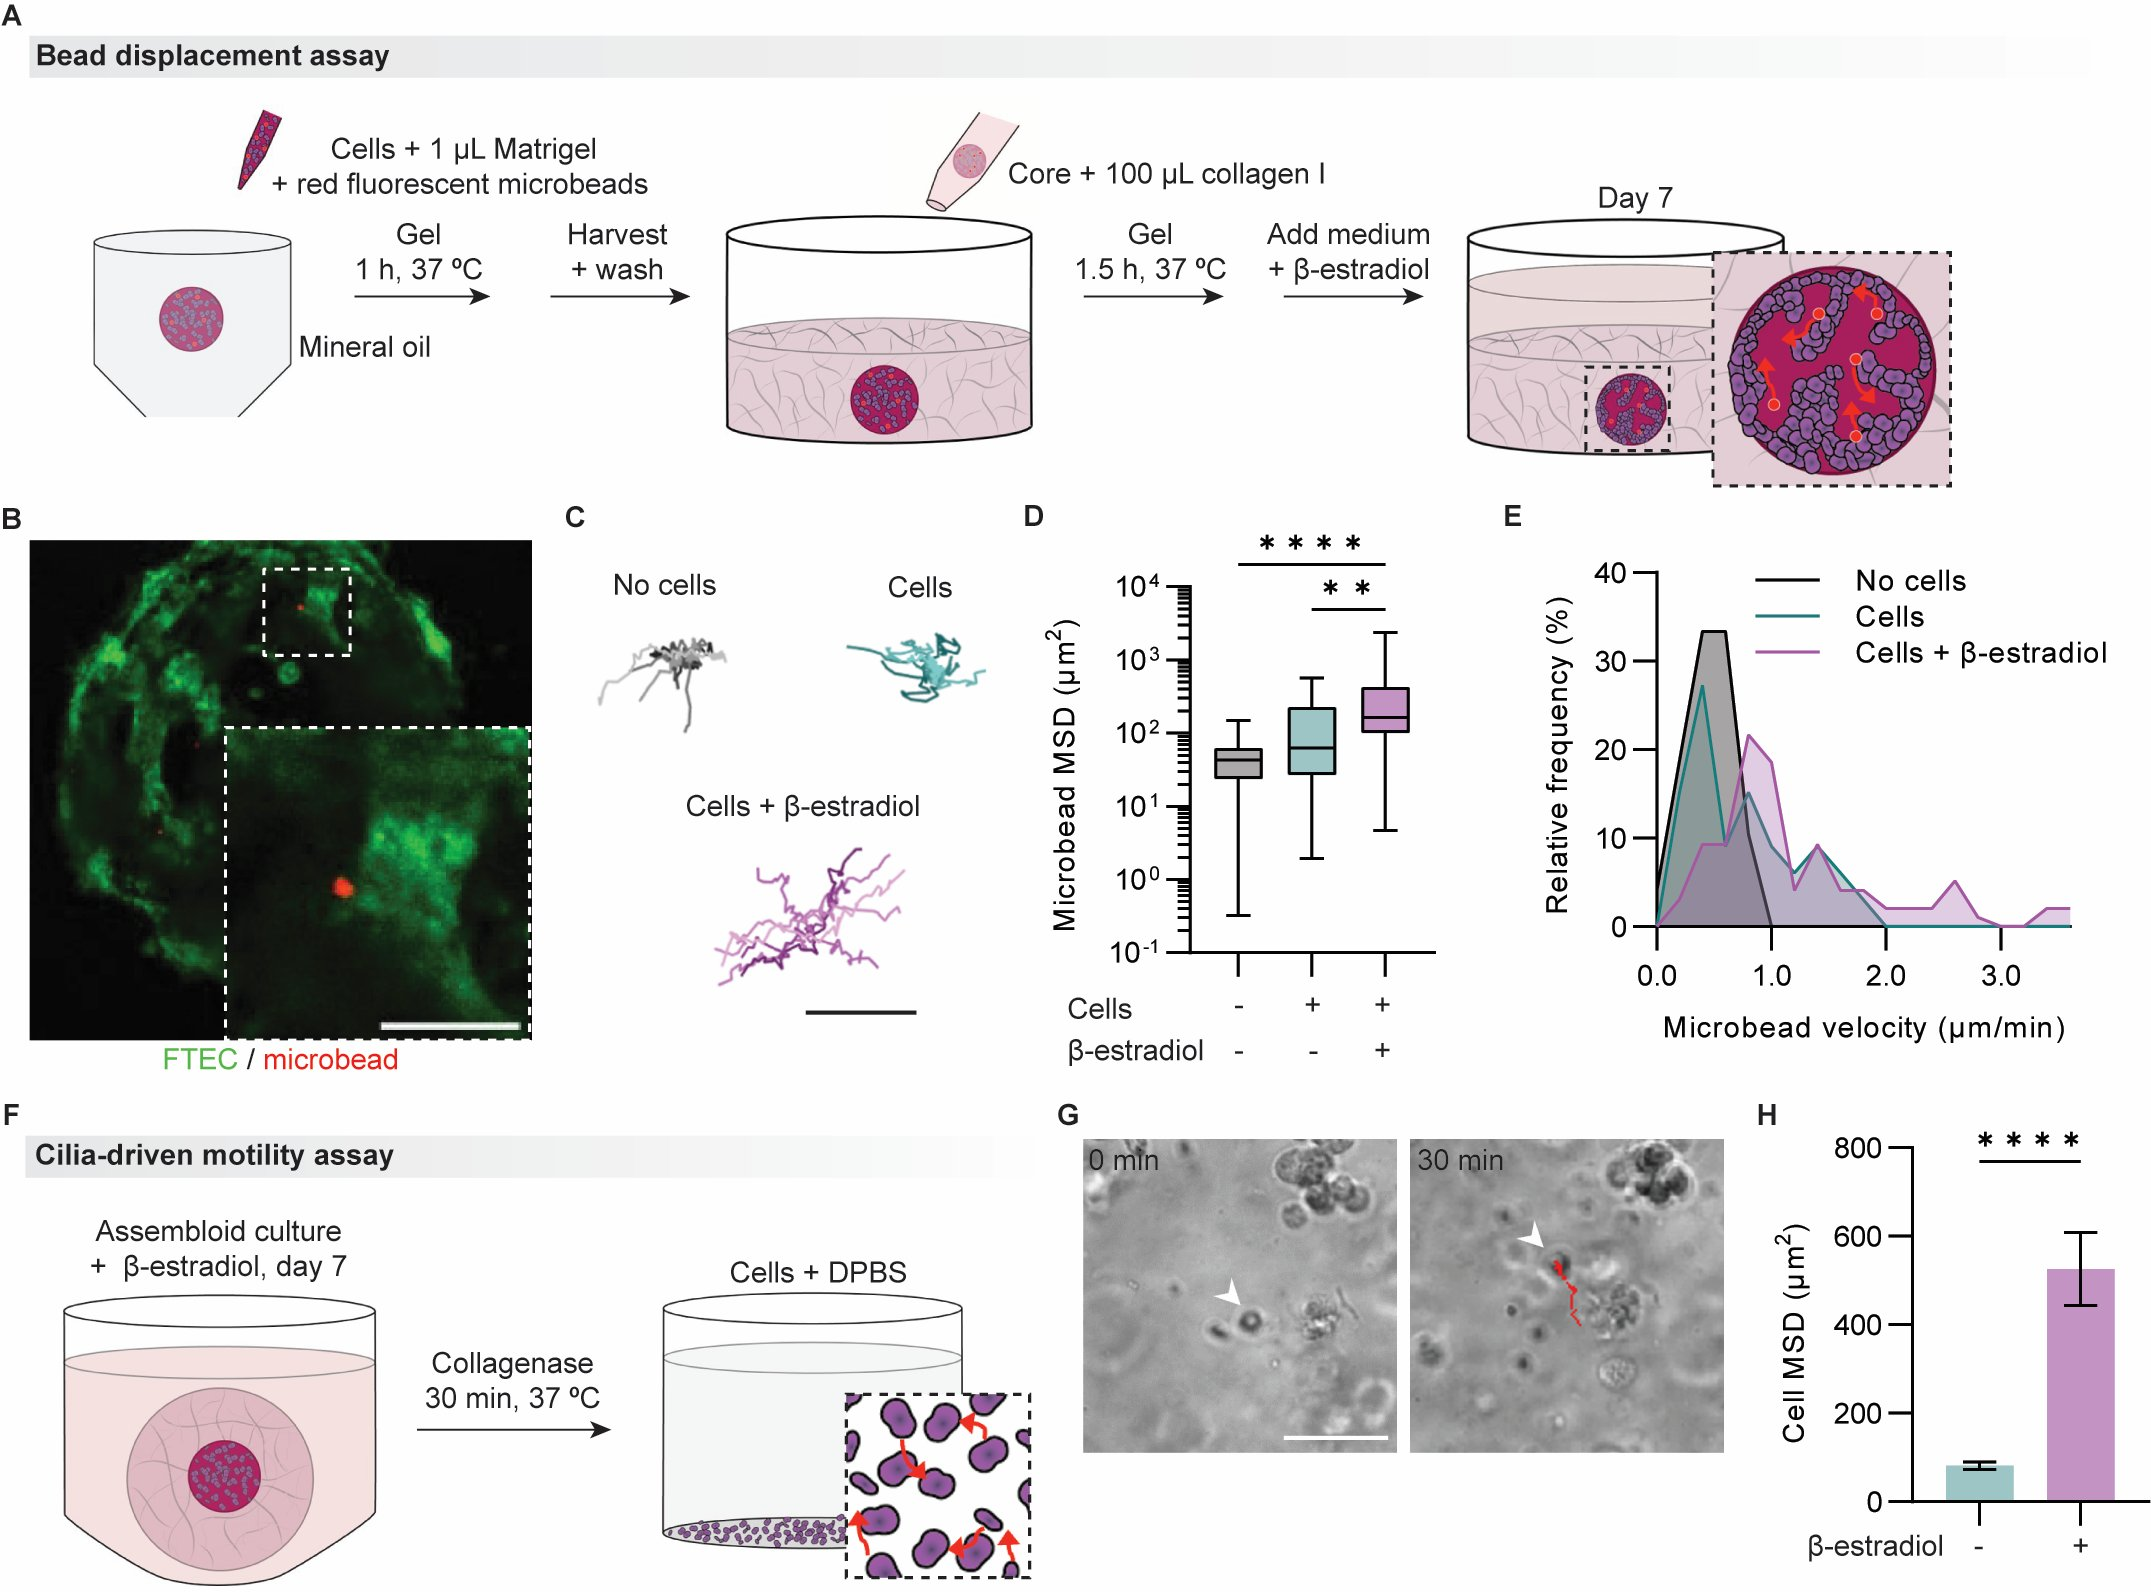
\includegraphics[width=1\textwidth,height=0.85\textheight,keepaspectratio,clip,page=1]{figures/chapter4/fig_4.jpg}
            \captionsetup{font=small}
            \caption{\textbf{Multi-compartment assembloids demonstrate functional similarity to the fallopian tube.} (A) Cartoon depicting the bead displacement assay protocol in assembloids. Arrows indicate microbead movement. (B) A multi-compartment assembloid used in the bead displacement assay with microbeads at the assembloid’s epithelial-lumen-like interface. EGFP-tagged FTECs (green) and microbeads (red). Scale bar, 100 µm. (C) Representative microbead trajectories from assembloid cores with microbeads only (noise, black), microbeads with FTECs (teal), and microbeads with FTECs treated with β-estradiol (purple). Scale bar, 10 µm. (D) Microbead MSDs over 8 h. Center line, median; box limits, upper and lower quartiles; whiskers, min to max. (E) Relative frequency of microbead velocities. (C)-(E) N = 3, n = 4-46. (F) Cartoon depicting cilia motility assay with assembloid digestion. Arrows indicate cell movement in DPBS. (G) Phase-contrast images from the cilia-driven motility assay. Cell trajectory (red). Scale bar, 50 µm. (H) Cell MSDs in DPBS after assembloid digestion. N = 3, n > 100. Statistical tests: (D) one-way ANOVA with multiple comparisons, (H) unpaired t-test, ****P ≤ 0.0001, **P ≤ 0.01. All data are mean ± SEM. }
            \label{chapter4_fig4}
        \end{center}
    \end{figure}
    
    % \begin{figure}[h!]
    %     \ContinuedFloat
    %     \captionsetup{font=small}
    %     \caption[]{}
    % \end{figure}

    \begin{figure}[p]
        \begin{center}
            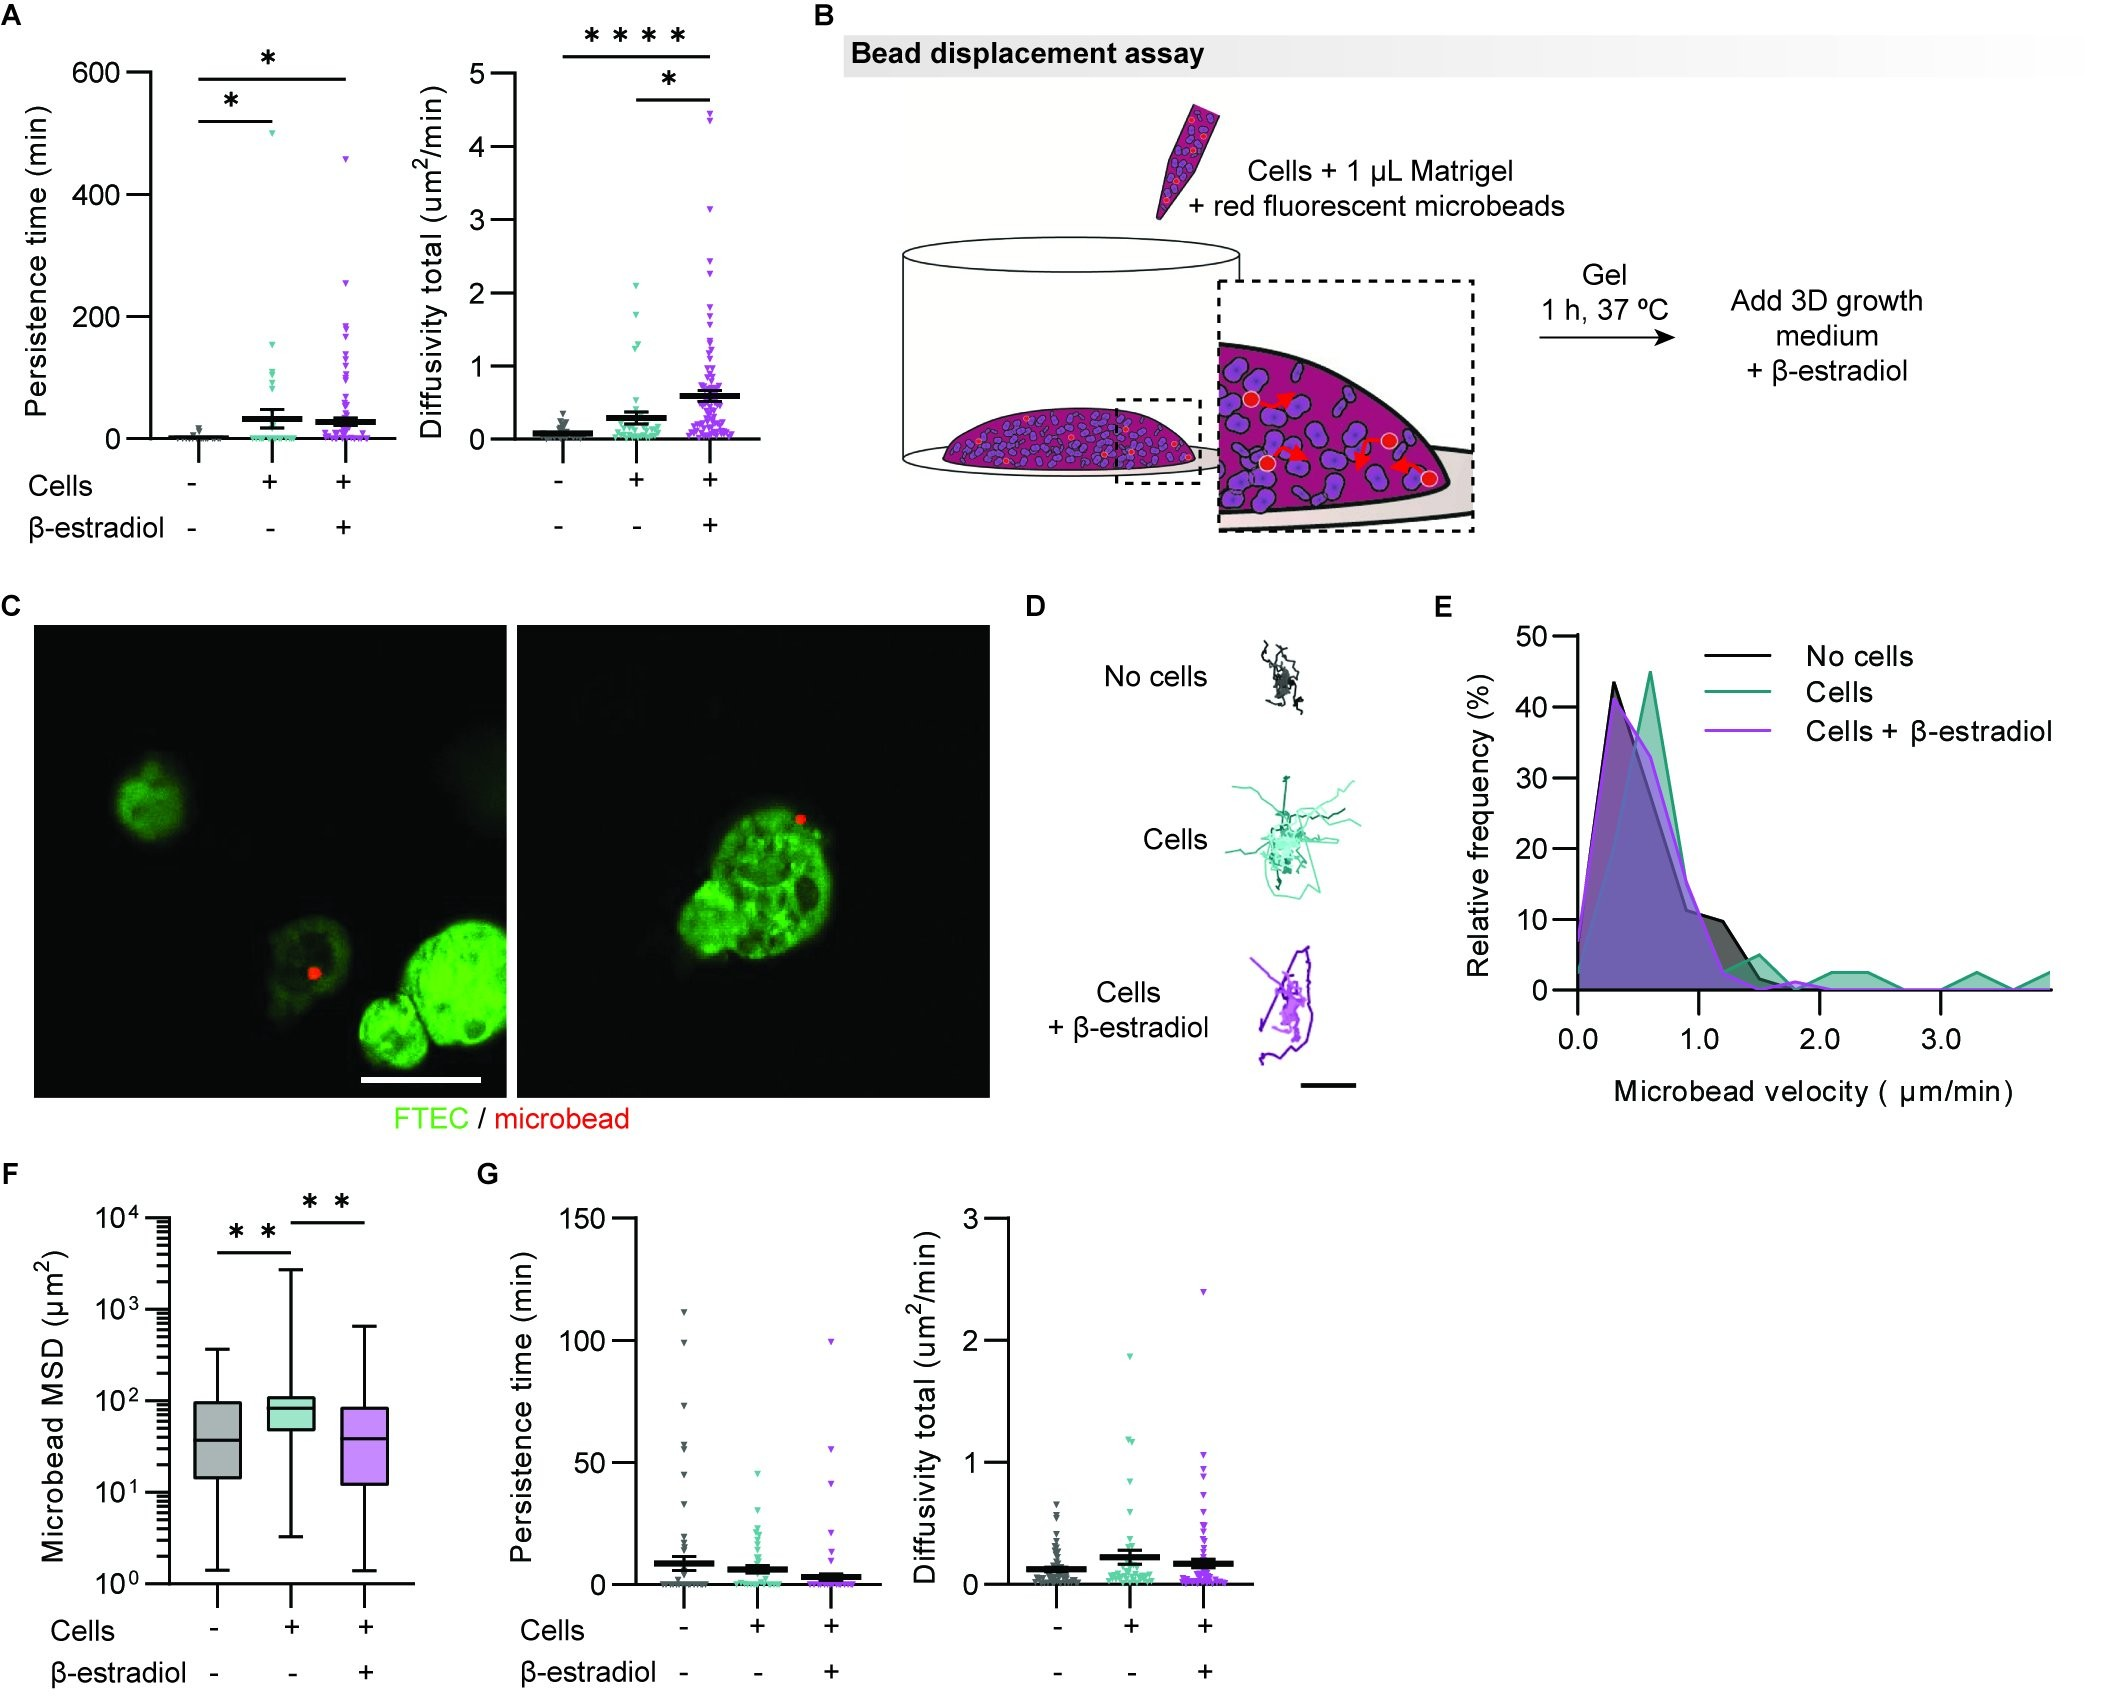
\includegraphics[width=1\textwidth,height=0.85\textheight,keepaspectratio,clip,page=1]{figures/chapter4/fig_S4.jpg}
            \captionsetup{font=small}
            \caption{\textbf{Mechanical function of ciliated epithelial cells.} (A) Persistence time and total diffusivity of microbeads in the multi-compartment bead displacement assay. N = 3, n = 4-46. (B) Cartoon depicting the bead displacement assay protocol in standard organoids. (C) A standard organoid used in the bead displacement assay with a microbead at the organoid’s epithelial interface. EGFP-tagged FTECs (green) and microbeads (red). Scale bar, 100 µm.(D) Representative microbead trajectories from standard organoids with microbeads only (noise, top), microbeads with FTECs (middle), and microbeads with FTECs treated with β-estradiol (bottom). Scale bar, 7.5 µm. (E) Relative frequency of microbead velocities in standard organoids. (F) Microbead MSD over 8 h. Center line, median; box limits, upper and lower quartiles; whiskers, min to max. (G) Persistence time and total diffusivity of microbeads in the standard organoid bead displacement assay. (D)-(G) N = 2, n = 18-45. (A) and (F)-(G) data are mean ± SEM. Statistical test: (A) and (F)-(G) one-way ANOVA with multiple comparisons, ****P ≤ 0.0001, **P ≤ 0.01, *P ≤ 0.05. }
            \label{chapter4_figS4}
        \end{center}
    \end{figure}
    
    % \begin{figure}[h!]
    %     \ContinuedFloat
    %     \captionsetup{font=small}
    %     \caption[]{}
    % \end{figure}
    
    \subsection{CODA provides architectural feedback for assembloid design iterations}
    After comprehensive evaluation of the multi-compartment assembloid model using traditional and novel in vitro assays, the assembloid model’s molecular and functional similarity to fallopian tube tissue was validated using quantitative metrics. The assembloid’s structure, however, was thus far evaluated using qualitative comparisons. To add quantitative validations of the 3D architecture of the multi-compartment assembloid, we developed a platform that rigorously compared our assembloids to a whole healthy human fallopian tube using CODA (Fig. 5A). CODA is a deep learning-based pipeline that 3D reconstructs bulk tissues at cellular resolution from serial histological sections\cite{kiemen2022a,Braxton20243D}. Here, CODA generated a 3D reference map of a whole fallopian tube received from a transplantation center from an organ donor who had no history of reproductive system disease or other history that would influence cellular architecture or function. Using this reference map, architectural measurements including the lumen volume and cell concentrations were quantified and then used to meticulously improve our assembloid model to best mimic the tissue architecture. Assembloid parameters were adjusted iteratively until this quantitative biomimetic comparison revealed marked improvement in structural biomimetic properties of our assembloid model (i.e., most quantifications were within 25\% deviation from the tissue).
    The CODA workflow was first applied to reconstruct the fallopian tube of a post-menopausal (72-year-old) female donor. Briefly, the FFPE tissue sample was serially sectioned (4 µm thickness) and one in every two sections was stained with hematoxylin and eosin (H\&E) and digitized for an axial resolution of 8 microns (Fig. 5B). We registered each H\&E image using nonlinear color image registration\cite{kiemen2022a} (Fig. 5C – panel a). Fallopian tube epithelium, stroma, and additional structures were labeled at a resolution of 1 micron using a semantic segmentation algorithm (Fig. 5C – panel b). Nucleus coordinates were generated through color deconvolution and detection of hematoxylin maxima, and validated through comparison with manually generated coordinates\cite{kiemen2022a} (Fig. 5C – panel c). This fallopian tube was assessed by a trained pathologist to ensure there were no pathological abnormalities and tissue labeling was accurate. Combination of registration, cell detection and tissue segmentation allowed for the production of 3D single-cell resolution maps (fig. S5A). Image alignment, tissue segmentation, and cell detection were all validated by a manually annotated ground truth (fig. S5B). We first produced a reference map of a whole healthy human fallopian tube that allowed us to visualize the intricate folding architecture of the epithelium-lumen interface in 3D (Fig. 5D). 
    The same CODA method was also applied to our assembloids to 3D reconstruct and label the assembloid epithelium and stroma (Fig. 5E) for a rigorous side-by-side comparison.  Multiple assembloids from the same generation were sectioned simultaneously from the same tissue block, but each assembloid was cropped from the histological slide scan and analyzed independently (Fig. 5B). Cellular and extracellular architectural quantifications were computed from tissue and assembloid maps to comprehensively compare their structures. We analyzed the level of similarity between organ and assembloid, adjusted assembloid parameters (ECM composition, cell seeding densities, addition of stromal cells), and repeated this process to produce a second generation (Fig. 5A). Additional assembloid parameters were adjusted as necessary to design subsequent assembloid generations. This iterative process concluded when the majority (four of six) of the architectural measurements were within 25\% deviation from the fallopian tube organ. 
    This hybrid CODA-assembloid platform demonstrates a novel validation process that combines advanced computational 3D mapping methods and advanced organoid/assembloid modeling to produce assembloids that closely mimic the microanatomy of the tissue of interest. It takes advantage of the versatility of our multi-compartment assembloid model. The result is an iteratively customized assembloid that closely resembles the reference fallopian tube. 

    \begin{figure}[p]
        \begin{center}
            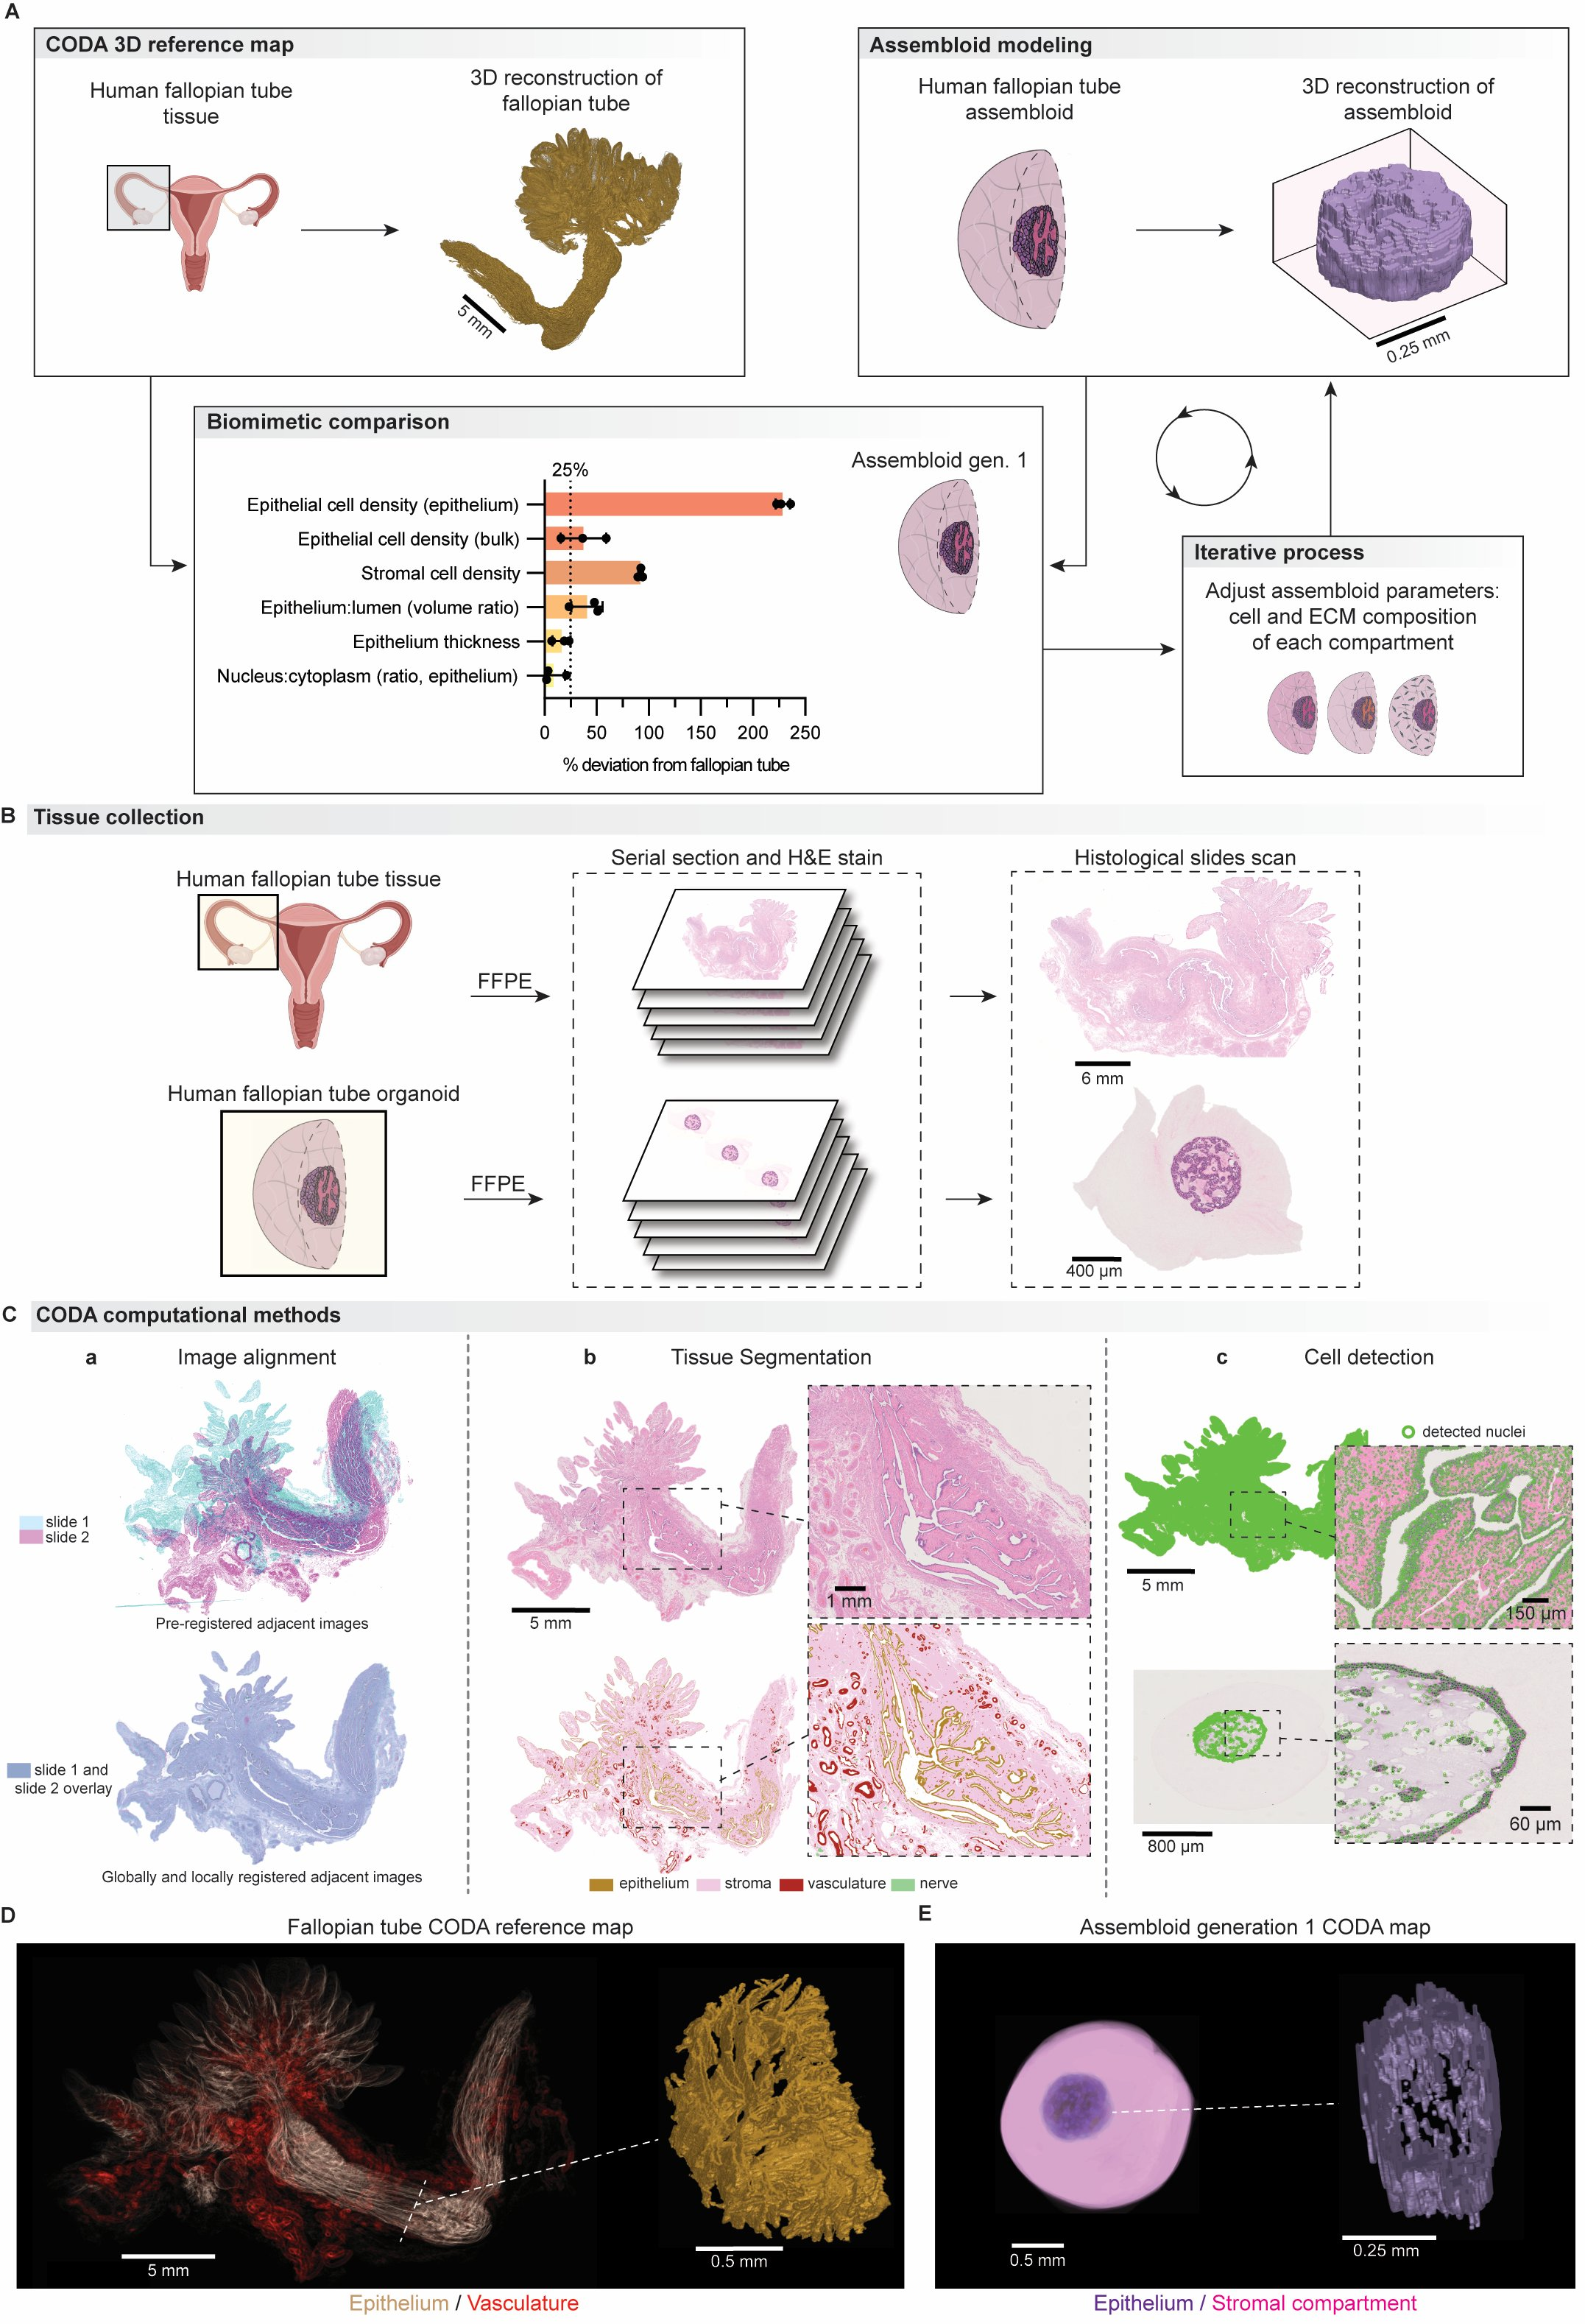
\includegraphics[width=1\textwidth,height=0.85\textheight,keepaspectratio,clip,page=1]{figures/chapter4/fig_5.jpg}
            \captionsetup{font=small}
            \caption{\textbf{Combined CODA and assembloid modeling in tandem produce a tissue-validated assembloid model.} (A) An iterative platform compared a tissue reference map (top left) and assembloid maps (top right). (Bottom left) Architectural quantifications were compared from these maps. (Bottom right) Assembloid parameters were adjusted and CODA imaging repeated until an assembloid generation closely matched the tissue architecture. }
            \label{chapter4_fig5}
        \end{center}
    \end{figure}
    
    \begin{figure}[h!]
        \ContinuedFloat
        \captionsetup{font=small}
        \caption[]{The CODA workflow: (B) Fallopian tube tissue and assembloids were formalin fixed, paraffin embedded (FFPE),  and the entire tissue was serial sectioned. One in every two tissue sections was stained with hematoxylin and eosin (H&E) and scanned at 20X magnification. (C) a, All scanned tissue sections were computationally aligned by an elastic registration process in sequential order. b, Tissue components such as the epithelium (gold), stroma (pink), vasculature (red) and nerves (green) were manually annotated in a small fraction of the images to train the deep learning algorithm to automatically segment all tissue sections. c, Individual cell nuclei were detected from the H&E images. Noise from image scans was adjusted in the cell count. (D) Z-projection of fallopian tube epithelium (gold) and vasculature (red) from a reference map. Scale bar, 5 mm. A 3D reconstruction of a cross section of the fallopian tube is shown (right). Scale bar, 0.5 mm. (E) Z-projection of the assembloid epithelium (purple) and stroma-like region (pink) from an assembloid map. Multi-compartment assembloid parameters: 1 x 104 FTECs in a growth factor reduced Matrigel core, 2 mg/mL collagen I corona. Scale bar, 0.5 mm. A 3D reconstruction of the assembloid epithelium is shown (right). Scale bar, 0.25 mm.}
    \end{figure}

    \begin{figure}[p]
        \begin{center}
            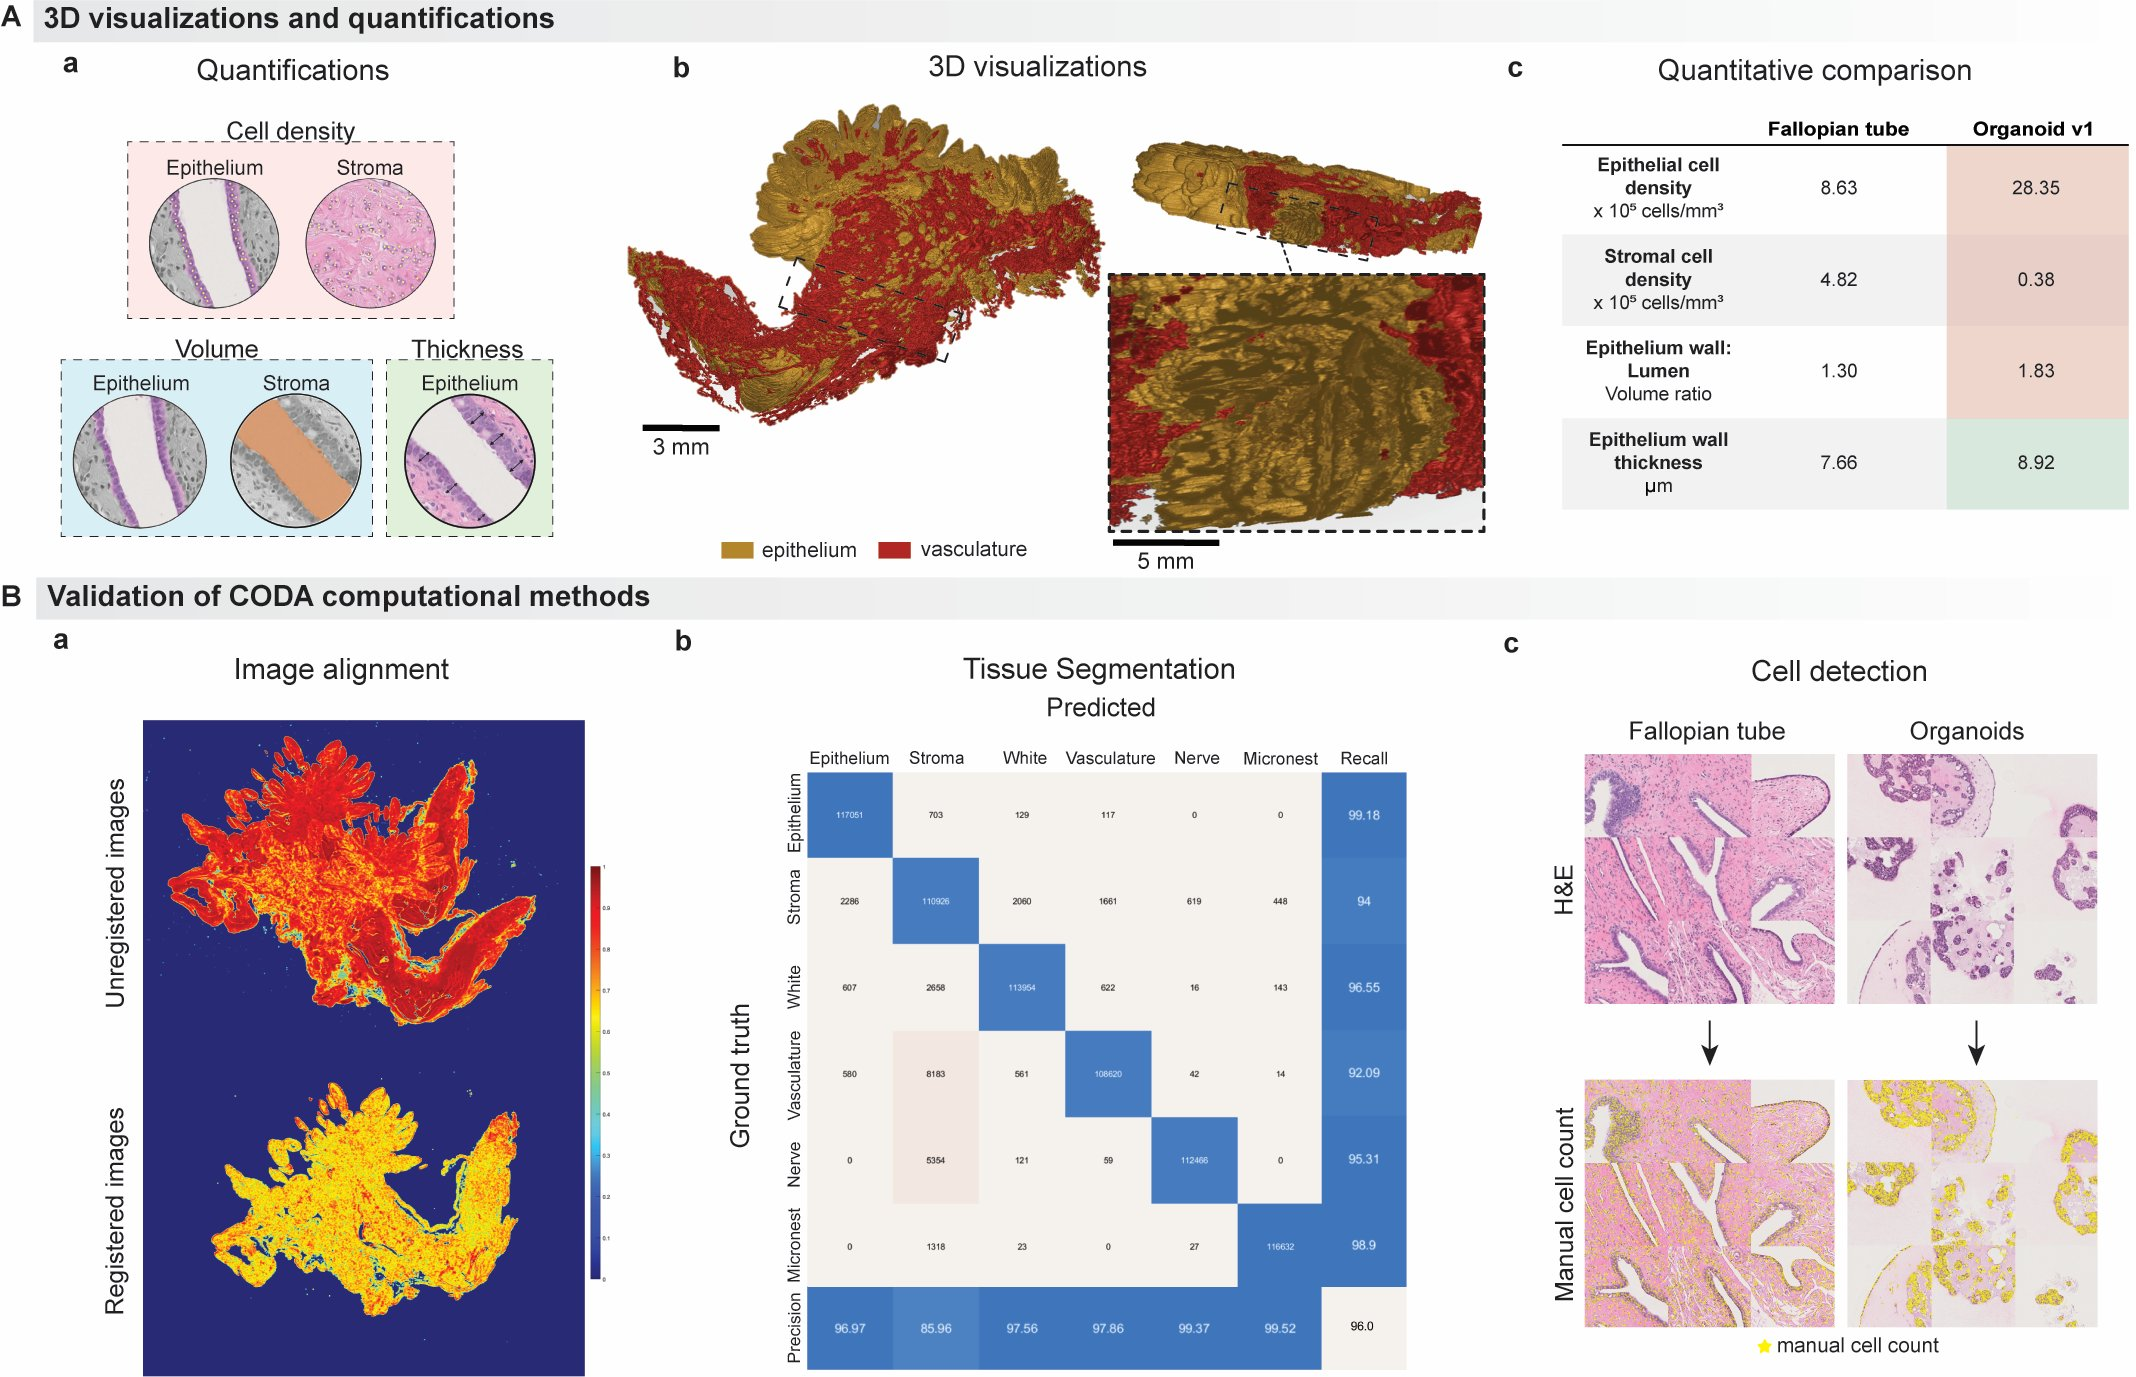
\includegraphics[width=1\textwidth,height=0.85\textheight,keepaspectratio,clip,page=1]{figures/chapter4/fig_S5.jpg}
            \captionsetup{font=small}
            \caption{\textbf{CODA post-processing.} (A) a, An array of tissue quantifications was measured from the processed tissue sections, and b, fallopian tube tissue and assembloids were visualized in 3D. Shown is an epithelium (gold) and vasculature (red) map of the fallopian tube. c, Architectural quantifications from each assembloid generation were compared to the tissue. (B) Independent testing of the CODA computational methods validated the performance of our reference maps, including a, image alignment, b, tissue segmentation, and c, cell detection.}
            \label{chapter4_figS5}
        \end{center}
    \end{figure}
    
    
    \subsection{Iterative changes to assembloid parameters converge towards a next-generation assembloid that mimics the fallopian tube architecture}
    CODA is a high resolution 3D tissue mapping technique, which we use here to improve our assembloid model; however, CODA is expensive, time-intensive, and requires specialized computational tools, making the technique medium throughput. To best leverage the insights gained from CODA maps, we chose seven different combinations of assembloid parameters including epithelial cell seeding densities, core Matrigel compositions, and corona collagen densities in addition to the standard organoid model (Fig. 6A, fig. S6A). These assembloids were not stimulated with β-estradiol to best reflect the post-menopausal conditions of the reference fallopian tube donor, where estrogen levels are low\cite{brodowska2021a,elmlinger2002a,andrew2022a} and fewer epithelial cells are ciliated\cite{crow1994a,donnez1985a,brodowska2021a}. Beginning with (1) the original assembloid parameters (1 x 10$^4$ epithelial cells seeded in a growth factor reduced Matrigel core and embedded in a 2 mg/mL collagen I corona), we first increased the collagen density in the assembloid corona (2) to 4 mg/mL and 6 mg/mL. Increasing the collagen density reduced the effect of epithelial cell contractility on shrinking the total size of the assembloid core, but did not significantly change the epithelial structure within the assembloid (Fig. 6A). We similarly changed the composition of the assembloid core ECM by seeding epithelial cells in a Matrigel matrix containing growth factors (3). This adjustment led to a change in the epithelial architecture where epithelial structures remained less connected within the assembloid core, as visualized by confocal microscopy. A similar difference in assembloid architecture was also observed when (4) decreasing the epithelial seeding in the assembloid core (5 x 10$^3$ cells seeded in a growth factor reduced Matrigel core and 2 mg/mL collagen corona) where the interconnected mucosal folding architecture again appeared less mature. 
    A unique advantage of the multi-compartment assembloid is that stromal cells can be added into the collagen-dense stroma-simulating corona (Fig. 6B). With this modification, we observed significant ECM remodeling when stromal cells were seeded in a 2 mg/mL collagen I corona, so we also increased the collagen concentration to 6 mg/mL (Fig. 6A, parameter modification 5). The standard organoid technique (6) was also imaged using CODA for a total of eight models that were analyzed using our architectural validation platform. Computational analysis was blinded to these experimental conditions.
    An array of structural quantifications were obtained from each assembloid map and compared to the CODA quantifications of the whole fallopian tube (Fig. 6C, fig. S6B). The measurements from this fallopian tube reference map focused on the ampulla region near the fimbriated end where a defined volume could be measured. This platform can be adjusted, however, to focus on different tissue regions and different arrays of architectural quantifications specific to the study. The epithelial and stromal cell seeding densities are two parameters of the assembloids that are easily adjusted, but have different impacts on the assembloid architecture. Cell density was calculated as a bulk measurement (epithelial cell count normalized by total assembloid volume) and as a packing density (epithelial cell count normalized by epithelial volume). While the epithelium cell density differed significantly from the reference tissue for all assembloid models when calculated as a packing density within only the organ/assembloid epithelium (Fig. 6D), the epithelial bulk cell density calculated across the whole assembloid more closely matched the tissue epithelial bulk density (Fig. 6E). 
    The inclusion of stromal cells had a significant impact on assembloid similarity to the tissue (Fig. 6F), which highlights the necessity of compartmentalization in an assembloid. Stromal cells can only be accurately incorporated into a fallopian tube assembloid model when they are adjacent to the epithelium and in direct contact with a collagen I matrix different from the epithelial ECM\cite{lengyel2022a}. Stromal cells were seeded at a ratio of 6 stromal cells to every 10 epithelial cells (6 x 10$^3$ stromal cells in the corona and 1 x 10$^4$ epithelial cells in the core). This seeding ratio accounted for the different proliferation rates of the cell types so that the final ratio of stromal cells to epithelial cells in mature assembloids closely matched the ratio counted in the tissue reference map (fig. S6B). The final number of stromal cells in mature assembloids was further modulated by collagen density in the corona. By increasing the collagen density from 2 mg/mL to 6 mg/mL, we decreased the final stromal cell count, which ultimately decreased the similarity of the stromal cell density per mm$^3$ total volume of our assembloid to the stromal cell density of the tissue within a 1 mm$^3$ region surrounding the fallopian tube lumen (Fig. 6F). Incorporating stromal cells into the assembloid corona also limited the proliferation of the assembloid epithelium (fig. S6C). 
    Additional quantifications included the epithelial wall volume and lumen volume, which was reported as a ratio to demonstrate the similarity of the relative scale of the assembloid to the relative scale of the reference fallopian tube (Fig. 6G). We also measured the thickness of the epithelium wall, which is an indicator of cellular organization (Fig. 6H). As shown in Fig. 6C, the fallopian tube epithelium can be a mixture of monolayered regions and regions where the epithelium becomes multi-layered. Here, we determined the average epithelium thickness across the whole organ epithelium and confirmed that the assembloid epithelium organized similarly. Finally, the nucleus to cytoplasm ratio of epithelial cells was measured so that we could compare the intracellular dimensions of epithelial cells to ensure these cells were not overpacking in the assembloid core (Fig. 6I).
    These quantifications for each assembloid generation were compared to the values for the reference fallopian tube by principal component analysis (PCA) (Fig. 6J). Each data point in the PCA plot represents a consolidation of multiple architectural quantifications derived from our CODA analysis, including epithelial and stromal cell densities, epithelial wall and lumen volume ratios, epithelium thickness, and nucleus to cytoplasm ratios presented above (Fig. 6D-I). This approach allows us to compare the structural similarity across different assembloid conditions and with the reference human fallopian tube tissue while simultaneously considering multiple parameters. The detailed measurements for each architectural feature used in this analysis are presented in Fig. S6B (Data S8), providing a comprehensive view of the data underlying each point in the PCA plot. PC1 and PC2 explained 34.75\% and 30.06\% of the total variance, respectively (PC3: 16.45\%, PC4: 12.72\%, PC5: 4.74\%, PC6: 1.28\%). This analysis revealed that the combination of seeding 1 x 104 FTECs in a growth factor reduced Matrigel core and embedding that core in a 2 mg/mL collagen I corona with 6 x 10$^3$ stromal cells (1 x 10$^4$ 2 mg/mL + S) best mimicked the reference fallopian tube tissue. The 1 x 10$^4$ 2 mg/mL + S condition stood apart from all other generations of the multi-compartment and standard organoid as a more accurate approximation of the fallopian tube architecture. The deviation between this assembloid and the reference fallopian tube was < 25\% for four of six architectural quantifications (Fig. 6F-I), thus this generation of multi-compartment assembloid achieved the target similarity to the reference fallopian tube. Finally, Euclidean distance analysis (fig. S6D), which gives equal weight to all metrics, also agreed that the similarity of the 1 x 10$^4$ 2 mg/mL + S condition to the reference fallopian tube was significantly improved compared to all other tested assembloid generations. The most distinguishing quantification was the stromal cell packing density, which was significantly improved in this assembloid generation. All assembloid parameters (1 x 10$^4$ epithelial cells seeded in growth factor reduced Matrigel with a 2 mg/mL collagen stroma) matched our molecularly and functionally validated assembloids with the only new addition of stromal cells into the corona. Via fluorescence confocal microscopy, we visualized in greater detail the architecture of this final assembloid generation (Fig. 6K, fig. S6E). Intricate epithelial folding mimicking the architecture of the fallopian tube mucosa was observed throughout the assembloid with a surrounding but distinct stroma-like region (Fig. 6L).
    
    \begin{figure}[p]
        \begin{center}
            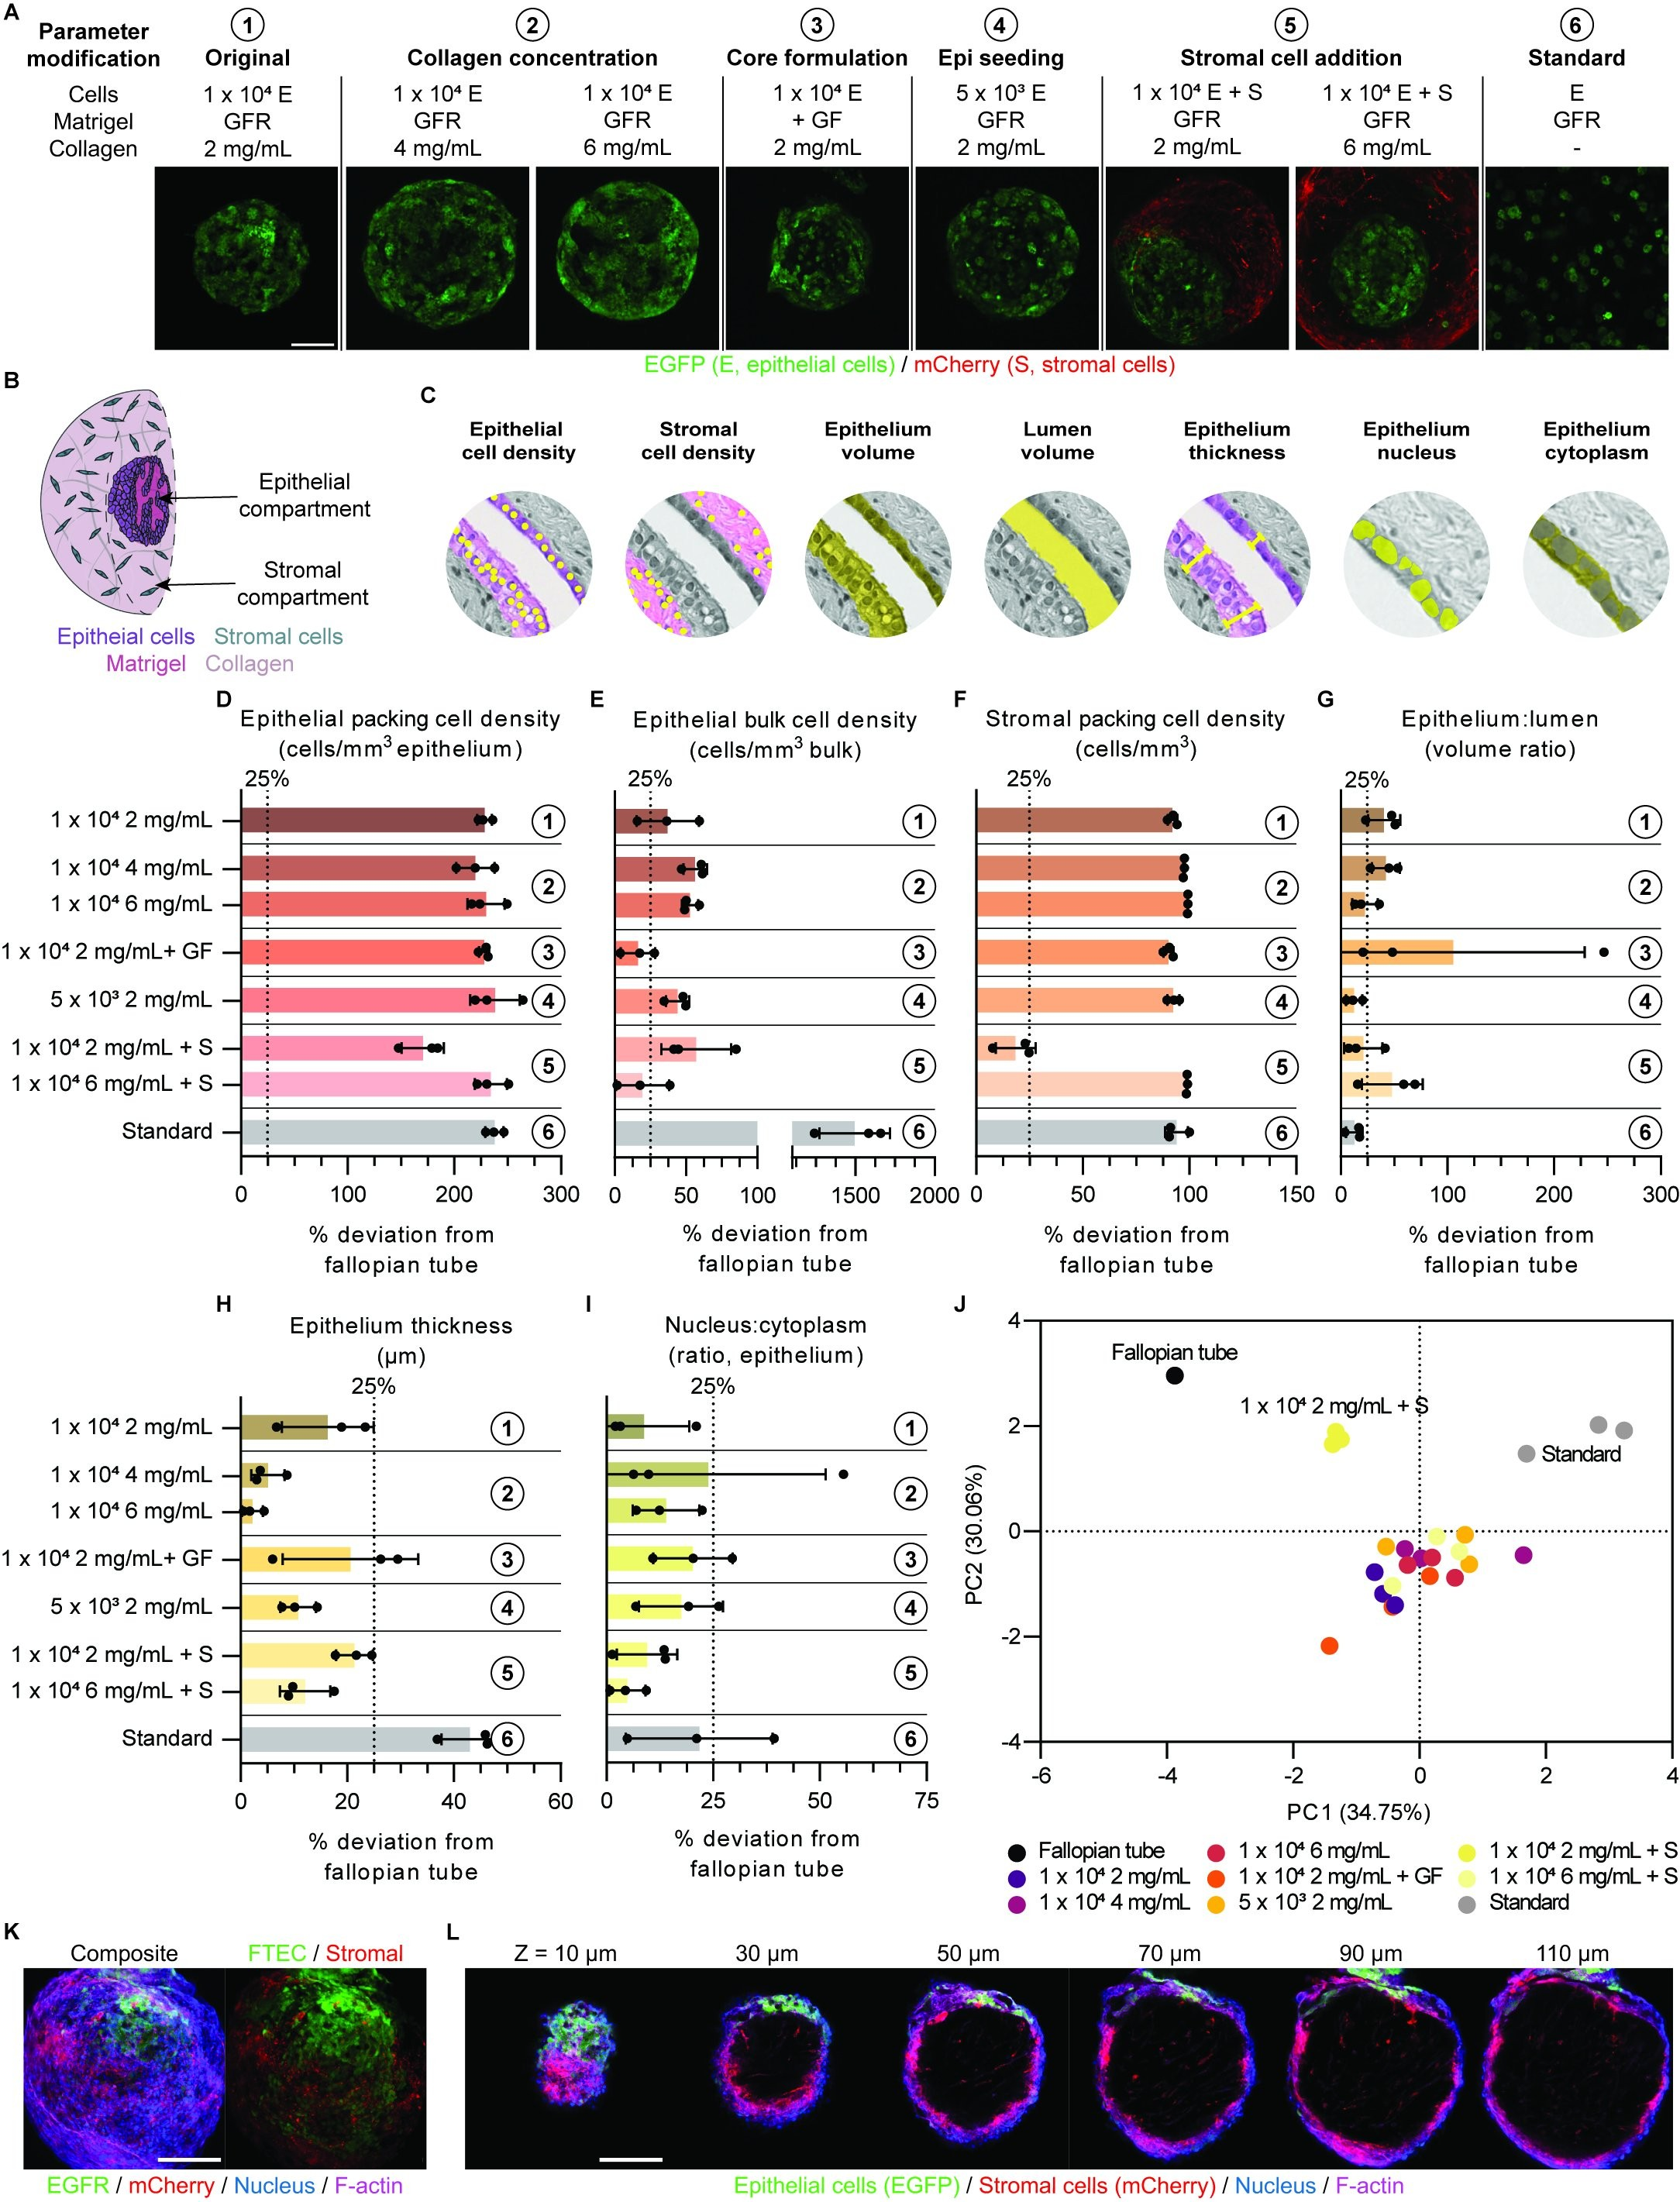
\includegraphics[width=1\textwidth,height=0.85\textheight,keepaspectratio,clip,page=1]{figures/chapter4/fig_6.jpg}
            \captionsetup{font=small}
            \caption{\textbf{Iterative changes to assembloid parameters produces a model that mimics the fallopian tube.} (A) Cell seeding numbers (1 x 10$^4$ or 5 x 10$^3$ cells/core), cell types (E = FTECs, S = stromal cells), Matrigel type (GFR = growth factor reduced, +GF = formulation with growth factors), and collagen density (2, 4, or 6 mg/mL) were adjusted in the multi-compartment model. Lines indicate a new parameter modification. Images are maximum intensity projections of stacks of fluorescence confocal microscopy images. EGFP-tagged FTECs (green) and mCherry-tagged stromal cells (red). Scale bar, 300 µm.}
            \label{chapter4_fig6}
        \end{center}
    \end{figure}
    
    \begin{figure}[h!]
        \ContinuedFloat
        \captionsetup{font=small}
        \caption[]{(B) Representative cartoon of the compartmentalization of epithelium and stroma within an assembloid. Epithelial cells (purple), stromal cells (blue), Matrigel (magenta), and collagen (pink). (C) Depictions of the architectural quantifications from CODA maps. The percent deviation of each assembloid generation from the fallopian tube reference values: (D) epithelial packing density within the epithelium wall only (cells/mm$^3$ epithelium), (E) epithelial bulk cell density across the whole tissue/assembloid (cells/mm$^3$ bulk), (F) stromal cell packing density within the stroma only (cells/mm3), (G) volume ratio of epithelium wall to lumen, (H) epithelium wall thickness (µm), and (I) ratio of epithelium nucleus to cytoplasm. Lines and numbering coordinate with parameter modifications. Dotted line indicates maximum target deviation (25\%). n = 3. Data are mean ± SD. (J) Quantitative comparison of assembloids to the healthy fallopian tube via PCA. Principal component \% proportion of variance listed. n = 3. (K) Maximum intensity projections of stacks of confocal fluorescence microscopy images of the 1 x 10$^4$ 2 mg/mL + S assembloid generation. FTEC (green), stromal cells (red), nuclear DNA (blue), F-actin (magenta). Scale bar, 200 µm. (L) Confocal fluorescence microscopy images of the 1 x 10$^4$ 2 mg/mL + S assembloid generation at varying heights throughout the assembloid. FTEC (green), stromal cells (red), nuclear DNA (blue), F-actin (magenta). Scale bar, 200 µm.}
    \end{figure}

    % \clearpage
    \FloatBarrier
    \subsection{Discussion}
    
    We demonstrate a tissue-informed assembloid engineering platform for the development and validation of in vitro models of organs with quantitative comparisons between the assembloid and the reference cellular map of the organ of interest. This multifaceted experimental, proteomics, and computational-based protocol can be applied to organoid/assembloid models of any tissue/organ and adapted to match the architectural, molecular, and functional parameters of the organ of interest. CODA-based analysis paired with multi-compartment assembloid modeling forms a robust platform that develops custom physiologically and anatomically accurate in vitro models. This platform enables the detailed study of the intricacies of many diseases and conditions. 
    This platform is demonstrated in the context of a healthy human fallopian tube as a basis for future studies of  gynecological conditions and diseases, such as HGSC and ectopic pregnancy\cite{shao2010a,chua2017a,labidi-galy2017a,jones2013a,kim2018a,ducie2017a}. We first demonstrated the structural similarity of our multi-compartment assembloid to the mucosal folding and ECM composition of the human fallopian tube following protocols that were previously used to validate the current state-of-the-art fallopian tube organoid model\cite{kessler2015a,xie2018a}. Second, the molecular similarity of our assembloid model to the fallopian tube was evaluated via comprehensive DIA-MS proteomics\cite{gillet2012a,collins2017a,bons2023a,meier2020a}. We measured the response of fallopian tube assembloids to female reproductive hormone stimulation via traditional functional assays\cite{kessler2015a,xie2018a,barton2020a} and developed a novel assay that measured the ability of the assembloid epithelium to actively transport an oocyte\cite{croxatto2002a,leese2001a,yuan2021a,suarez2021a,wanggren2008a}. Through these two functional assays, the multi-compartment assembloid mimicked the molecular and mechanical functions of the fallopian tube. Finally, we directly compared the multi-compartment assembloid architecture to a reference fallopian tube using quantitative metrics via CODA\cite{kiemen2022a}. Design parameters of the multi-compartment assembloid were customized to best match the post-menopausal conditions of this reference organ through iterative adjustments to assembloid design parameters and sequential CODA mapping. Through this comprehensive analysis, our multi-compartment assembloid demonstrated physiological similarity to the fallopian tube via molecular, functional, and architectural assessments.
    Customizing an assembloid model with reference to the architecture of a whole, transplantation-quality human organ provides an additional quantitative validation of the assembloid model. To our knowledge, direct 3D and quantitative comparison of in vitro cell culture models to organ microarchitecture and cellular composition has never been performed for fallopian tube or other organoid/assembloid models, although the field of in vitro modeling has recognized the importance of validation through other histopathology and tissue-omics-based approaches\cite{garcia-alonso2021a,camp2018a,zhao2022a}. The complex heterogeneity of tissues can only be revealed in 3D\cite{kiemen2022a,Forjaz2025Three}, hence our prioritization of 3D CODA mapping over conventional histological analysis (2D).
    As parameters of our multi-compartment fallopian tube assembloid were modulated, CODA imaging and architectural quantification identified an optimized combination of assembloid parameters. The epithelial and ECM composition of this optimized assembloid design (1 x 104 epithelial cells seeded in growth factor reduced Matrigel with a 2 mg/mL collagen stroma) matched our initial design parameters that we validated via molecular and functional assays. The importance of a secondary compartment was strengthened by the CODA-based platform identifying the addition of stromal cells in the corona (1 x 10$^4$ seeded in growth factor reduced Matrigel with a 2 mg/mL collagen stroma containing 6 x 10$^3$ stromal cells) as the only modification to these original assembloid design parameters to significantly enhance the accuracy of the fallopian tube assembloid architecture. Stromal cells can only be physiologically added to such assembloid models when isolated from epithelial cells in a collagen-rich ECM, which necessitates a multi-compartment model. While ideally, all structural, molecular, and functional assays would be performed using this optimized version of the assembloid, limitations of the system make the molecular and functional assays difficult to perform in a coculture model. Adding stromal cells to the collagen compartment makes the corona more opaque and more difficult to image at significant depths into the assembloid using light-based microscopy methods. Molecular assessments are complicated by sample loss and loss of 3D cell-cell or cell-ECM interactions when attempting to harvest cell types individually for molecular assays. Our bead displacement assay testing the mechanical function of the fallopian tube epithelium to transport an object was also difficult to perform in the coculture system. Time-lapse imaging of the same location is required, but the whole assembloid shifts significantly when stromal cells are reorganizing the collagen compartment. For these reasons, we relied on the closest approximation to our CODA optimized assembloid parameters (1 x 10$^4$ seeded in growth factor reduced Matrigel with a 2 mg/mL collagen stroma) for our molecular and functional assessments.
    The use of customizable multi-compartment assembloids allows us to decipher some of the key compositional features that support the maturation, controlled growth, and maintenance of fallopian tubes. This work establishes the critical importance of two physiological extracellular matrices (i.e., a basement membrane and surrounding collagen compartment)\cite{wheeler1982a,popescu2005a} for FTECs to organize into mucosal folds and stimulate the production of additional ECM proteins that match the ECM composition of the human fallopian tube\cite{shao2023a}. This ECM composition can introduce a limitation of the multi-compartment assembloid system where the lumen-like region is filled with Matrigel (basement membrane) when the true fallopian tube architecture contains a hollow lumen. However, such physiological cell-ECM interactions are necessary to polarize FTECs such that both ciliated and secretory cells face the lumen-like region\cite{popescu2005a,kessler2015a} where ciliated cells could reproduce the organ’s mechanical function and transport an oocyte\cite{yuan2021a,suarez2021a,wanggren2008a}. We also establish the critical importance of stromal cells in a secondary compartment, as observed in fallopian tube tissue\cite{wheeler1982a}, to limit epithelial growth, so that the mucosal folding architecture could be maintained over long time scales. 
    Our multi-compartment assembloid model of the human fallopian tube is a tissue-validated, healthy model. In future work, the cell-cell and cell-ECM interactions in the assembloid model can also be customized to reflect diseased tissues (e.g., precursor lesions to HGSC\cite{kuhn2012a}) and referenced back to corresponding diseased tissue CODA maps via the iterative platform we demonstrated here.  These studies could include altering the ECM composition\cite{rentchler2019a} and healthy vs. p53 signature cell ratios in the epithelium\cite{shih2021a}, or investigations of cilia-driven transport of developing oocytes in tubal pregnancy\cite{shao2010a,chua2017a}.  Other studies of the role of hormone changes in successful embryo implantation are also possible as HSPG2 and other protein expression levels were tunable through \textbeta-estradiol stimulation in the multi-compartment model\cite{chen2023a,garcia2024a}.  The versatility of this approach provides the opportunity to include additional cell mechanical interactions or introduce disease-related ECM changes in downstream experimental applications, or to apply similar 3D culture, proteomics-based, and CODA mapping techniques to evaluate the physiological accuracy of in vitro models of other human tissues. Through our iterative process, we produced a quantitatively optimized and functional assembloid model of a human fallopian tube. This assembloid validation platform can be applied to any tissue-organoid or tissue-assembloid pair to determine the biological accuracy of in vitro models.
    
    \section{Materials and Methods}
    \subsection{Fallopian tube tissue}
    Whole healthy fallopian tube tissues were received from organ procurement organizations from donors with no history of disease. All procedures were approved by the Johns Hopkins Internal Review Board (IRB00324065). The tissues were transported in saline on wet ice, formalin fixed (10\%, VWR 16004-121) and paraffin embedded. The entire tissue was serial sectioned at 4 µm thickness at Johns Hopkins Oncology Tissue Services (SKCC). Tissue sections were stained with hematoxylin and eosin, or immunohistochemistry (IHC) stained. Antibodies used in IHC staining are listed in table S1. Tissue sections were scanned at 20X or 40X magnification (Hamamatsu NanoZoomer S210).
    
    \subsection{Cell culture}
    Fallopian tube immortalized cells were the FT2821J (epithelial)\cite{park2021a,wang2022a,jung2014a,song2019a}, FT194 (epithelial, CVCL-A4AW)\cite{wang2022a} and hS1 (fibroblast-like stromal)\cite{park2021a} cell lines. Cells were cultured in RPMI 1640 (Gibco 11875-093) with 10\% FBS (Corning 35-010-CV) and 1\% penicillin-streptomycin (Sigma P0781). Fallopian tube primary epithelial cells (LifeLine Cell Technology FC-0081) were validated and quality tested at LifeLine Cell Technology and cultured in complete ReproLifeTM Reproductive Medium (LifeLine Cell Technology LL-0068) for a maximum of 3 passages. All cells were cultured at 37°C and 5\% CO2 in a humidified incubator and did not surpass 20 cell passages. All experiments were conducted using these base culture mediums for immortalized or primary cells.
    Fluorescently tagged cells were transduced via lentivirus delivery of the fluorescent tag. Luciferase expressing cells were transduced via lentivirus delivery of a luciferase-mCherry tag (pSLCAR-CD19-BBz [Addgene 135992] with luciferase [Addgene 46793] and mCherry [Addgene 84020] sequences inserted). Transduced populations were expanded and sorted by fluorescence-activated cell sorting (SONY SH800).
    
    \subsection{Multi-compartment assembloid}
    The protocol for generating multi-compartment assembloids is described in greater detail by Lee, et al., where the protocol was first established as a tumor organoid model\cite{lee2022a}. In short, a single-cell suspension of 1 x 104 or 5 x 103 fallopian tube epithelial cells per µL Matrigel (standard formulation 354234 or growth factor reduced 354230, Corning) were pipetted in 1 µL volumes in columns (USA Scientific 1111-3700) containing mineral oil (Sigma 69794) and allowed to gel at 37°C. After 1 h, these cores were collected in cell culture medium (RPMI 1640, Gibco 11875-093) to wash off the mineral oil and embedded in collagen I (high concentration rat tail type I, Corning 354249). A final concentration of 2, 4 or 6 mg/mL collagen I was used according to a previously described protocol (101–104). Adjustments to the collagen I concentration in the assembloid corona were made to assess the effects of corona composition on assembloid architectural similarity to fallopian tube tissue, or to support longer-term cultures of fallopian tube epithelial cells.  Drops containing one assembloid core and 10 µL of collagen I were pipetted into fresh mineral oil columns and again allowed to gel at 37°C. After 1.5 h, these assembloids were collected in cell culture medium to wash off any remaining mineral oil and plated in a 96-well round bottom plate (Genesee Scientific 25-224) with normal cell culture medium as described above. All assembloids were cultured at 37°C and 5\% CO2 in a humidified incubator. All assembloids were grown for at least 6 days (immortalized FTECs) or 9 days (primary FTECs) to allow time for the epithelial architectures to mature. These multi-compartment assembloids are medium throughput, generating up to 96 assembloids per batch.  The consistency of size control across batches was measured using NIS Elements software.
    
    \subsection{Standard organoid}
    The protocol for generating standard organoid is described in greater detail by Kessler, et al. (28) Briefly, fallopian tube epithelial cells were suspended in growth factor reduced Matrigel (Corning 354230) at 500 cells/µL. 50µL drops of the mixture were plated on a glass bottom plate and allowed to gel. Organoids were grown in organoid formation medium containing Advanced DMEM/F-12 (Gibco 12634010), L-Glutamine (1\%, Gibco 25030081), B-27 (2\%, Gibco 17504044), EGF (0.1 µg/mL, ThermoFisher PHG0311), Y-27632 ROCK Inhibitor (10 µM, Cayman Chemical 10005583), TGF-\textbeta RI Kinase Inhibitor VI SB431542 (0.5 µM, Sigma 616464) and HEPES (1\%, Gibco 15630080). All organoids were cultured at 37°C and 5\% CO2 in a humidified incubator. Timelines used for standard organoids matched the culture timelines of multi-compartment assembloids.
    \subsection{PrestoBlue proliferation assay}
    Assembloid total proliferation was assessed via the PrestoBlue (ThermoFisher A13262) proliferation assay. Assembloids were incubated with PrestoBlue (10X) diluted to 1X in culture medium for 3 h at 37°C and 5\% CO$^2$ in a humidified incubator. Red fluorescence (RFU) was read on a SpectraMax plate reader (Molecular Devices, excitation 540, emission 600, cutoff 590). The average of at least 3 background wells of 1X PrestoBlue diluted in culture medium without assembloids was subtracted from all RFU values. PrestoBlue solution was washed from assembloids by replenishing culture medium twice with DPBS (Corning 21-031-CV) and twice with culture medium, and cultured until the next timepoint at 37°C and 5\% CO2 in a humidified incubator.
    
    \subsection{Imaging}
    Assembloids and organoids were imaged on a Nikon Ti2 microscope (phase-contrast) and a Nikon A1R confocal/Nikon Eclipse Ti inverted microscope (DIC, fluorescence and immunofluorescence confocal). The Nikon Ti2 microscope was equipped with a DS-Qi2 camera and a 10X/0.30 Plan Fluor Ph1 DL objective (Nikon). Temperature and CO$^2$ were controlled with a Tokai Hit stage top incubator. The Nikon A1R confocal/Nikon Eclipse Ti inverted microscope was equipped with a 10X/0.30 DIC L/N1 and 20X/10.75 DIC M/N2 Plan Fluor objective (Nikon), a 10X and 20X DIC slider (Nikon), and a N1 and N2 DIC condenser (Nikon). Temperature and CO$^2$ were controlled with an OKO Labs stage top incubator.
    Fluorescence and immunofluorescence confocal images are maximum intensity projections of z-stacks taken over 200-500 µm height of the assembloid with a 10 µm interval. Assembloids were fixed overnight in 4\% PFA or grown in a glass bottom plate for imaging (EGFP, mCherry). Nuclei were stained with Hoechst 33342 (ThermoFisher H3570) and F-actin was stained with Phalloidin 488 (Invitrogen A12379) or Phalloidin 647 (Invitrogen A22287) for 1 h. The primary and secondary antibodies used in immunofluorescence (IF) imaging are outlined in table S1. For IF studies, assembloids were permeabilized in 0.1\% Triton X-100 (Sigma T9284) in DPBS (Corning 21-031-CV) for 1 h, blocked with 5\% normal goat serum (NGS, Cell Signaling Technology) in DPBS for 3 h, and primary stained overnight in 1\% NGS in DPBS. Assembloids were secondary stained for 3 h in 1\% NGS in DPBS. Assembloids were cleared for 20 minutes in a fructose-glycerol clearing solution (105) (60\% glycerol [JT Baker 2136-03], 2.5M D-fructose [Sigma F0127] in DI water) and imaged in DPBS or clearing solution. 

    \begin{table}[htbp]
        \centering
        \footnotesize % Smaller font for the table
        \renewcommand{\arraystretch}{1.2} % Adjust row height
        \caption{Antibodies used in immunofluorescence (IF), immunohistochemistry (IHC), and western blots (WB).}
        \label{chapter4_table_S1}
        \begin{tabularx}{\textwidth}{l l l l}
            \toprule
            \textbf{Application} & \textbf{Antibody} & \textbf{Company} & \textbf{Product \#} \\
            \midrule
            IF  & E-cadherin                  & Cell Signaling Technology & 3195  \\
            IF  & Ki-67                      & Cell Signaling Technology & 9449  \\
            IF  & PAX8                       & Cell Signaling Technology & 59019 \\
            IF  & MUC16                      & Cell Signaling Technology & 29623 \\
            IF  & Anti-rabbit IgG, Alexa Fluor 568 & Invitrogen        & A-11011 \\
            IF  & Anti-mouse IgG, Alexa Fluor 568  & Invitrogen        & A-11004 \\
            IHC & E-cadherin                  & Cell Signaling Technology & 3195  \\
            IHC & Ki-67                      & Abcam                    & ab16667 \\
            IHC & PAX8                       & Cell Signaling Technology & 28556 \\
            WB  & E-cadherin                  & Cell Signaling Technology & 3195  \\
            WB  & Occludin                   & Cell Signaling Technology & 91131 \\
            WB  & GAPDH                      & Cell Signaling Technology & 2118  \\
            WB  & Anti-rabbit IgG, HRP-linked & Cell Signaling Technology & 7074  \\
            \bottomrule
        \end{tabularx}
    \end{table}
    
    \subsection{Transmission electron microscopy}
    Assembloids were fixed (2.5\% glutaraldehyde, 0.1M sodium cacolydate buffer, 3 mM magnesium chloride in DI water), and imaged via transmission electron microscopy. Images were captured and analyzed with the help of a transmission electron microscopy expert at the Johns Hopkins School of Medicine Microscope Facility.
    
    \subsection{Western blot}
    Protein was extracted from 3D cultures and 2D cells with 2X clear sample buffer (120 mM Tris pH 6.8, 4\% SDS, 20\% glycerol) and 1X protease/phosphatase inhibitor (Cell Signaling Technology 5872). 2D cells were scraped from a 10 cm dish after coating the plate with 2X clear sample buffer. All protein samples were sonicated with a needle probe sonicator (10-15 pulses, VWR Scientific) and denatured at 100°C for 5 minutes. Samples were stored at -80°C. Protein concentration was measured by microBCA (ThermoFisher, 23235) and absorbance measured on a SpectraMax plate reader (Molecular Devices, 562nm). Samples were diluted to 1 µg/µL in 2X Lamelli (BioRad 1610737) and heated for 5 minutes at 100°C. Samples were loaded in a 4-15\% mini-protean gel (BioRad 4561086) for gel electrophoresis (BioRad PowerPac). Protein bands were transferred to a PVDF membrane using a Transblot Turbo pack (BioRad 1704156). The blot was blocked in blotting-grade blocker (5\%, 1706404) in TBST (1X Tris Buffered Saline [BioRad 1706435], 0.1\% Tween 20 [Sigma P1379], in DI water) for 1 h and primary stained overnight at 4°C. HRP-conjugated secondary antibodies were incubated at room temperature for 1 h. Western blots were imaged on a BioRad ChemiDoc XRS+ imager with Prometheus™ ProSignal™ HRP substrate (Genesee Scientific 20-302). Antibodies are listed in table S1. 
    \subsection{Hormone stimulation and RT-qPCR}
    After 7 days of culture, assembloid architecture had matured, and assembloids/organoids were treated with \textbeta-estradiol (E2, 500 pmol/L, Sigma E2758), progesterone (P4, 50 ng/mL, Fisher Scientific AC225650250)\cite{kessler2015a}, or an untreated control. Hormones were diluted in ethanol prior to dilution in culture medium, so this dilution was equivalently reflected in the untreated control. Assembloids and organoids were grown for another 7 days with hormone stimulation before mRNA harvested (Zymo Research R2052 Direct-zol RNA MiniPrep 11-331) and cDNA synthesized using the iScript™ cDNA Synthesis Kit (BioRad 1708891) and a Blue-Ray Biotech thermocycler. Expression of select genes (primers from Integrated DNA Technologies listed in table S2)\cite{kessler2015a,xie2018a,ma2022a,rajurkar2017a,liu2020a} was quantified by iTaq-SYBR Green (BioRad) RT-qPCR on a BioRad CFX384 Touch Real-Time PCR detection system. Relative expression was calculated according to the equations described by Pfaffl\cite{pfaffl2001a}.

    \begin{table}[htbp]
        \centering
        \footnotesize
        \renewcommand{\arraystretch}{1.2}
        \caption{Primers used in RT-qPCR.}
        \label{chapter4_table_S2}
        \begin{tabularx}{\textwidth}{l l X} % X column automatically adjusts width
            \toprule
            \textbf{Gene} & \textbf{FWD/RVS} & \textbf{Sequence} \\
            \midrule
            PAX8   & FWD & AAGTGCAGCAACCATTCAACC \\
            PAX8   & RVS & CTGCTCTGTGAGTCAATGCTTA \\
            FOXJ1  & FWD & GGAGGGGACGTAAATCCCTA \\
            FOXJ1  & RVS & GGTCCCAGTAGTTCCAGCAA \\
            OVGP1  & FWD & TCCCACACATCGTCCAAACAT \\
            OVGP1  & RVS & TCCCCATGATGAGCTTCTCTG \\
            OLFM4  & FWD & ACTGTCCGAATTGACATCATGG \\
            OLFM4  & RVS & TTCTGAGCTTCCACCAAAACTC \\
            MKI67  & FWD & AAGCCCTCCAGCTCCTAGTC \\
            MKI67  & RVS & TCCGAAGCACCACTTCTTCT \\
            TNF    & FWD & CCTCTCTCTAATCAGCCCTCTG \\
            TNF    & RVS & GAGGACCTGGGAGTAGATGAG \\
            ESR1   & FWD & CCCACTCAACAGCGTGTCTC \\
            ESR1   & RVS & CGTCGATTATCTGAATTTGGCCT \\
            PGR    & FWD & ACCCGCCCTATCTCAACTACC \\
            PGR    & RVS & AGGACACCATAATGACAGCCT \\
            18S    & FWD & AGAAGTGACGCAGCCCTCTA \\
            18S    & RVS & GAGGATGAGGTGGAACGTGT \\
            ATUB   & FWD & AGGAGTCCAGATCGGCAATG \\
            ATUB   & RVS & GTCCCCACCACCAATGGTTT \\
            ACTB   & FWD & CATGTACGTTGCTATCCAGGC \\
            ACTB   & RVS & CTCCTTAATGTCACGCACGAT \\
            GAPDH  & FWD & GGAGCGAGATCCCTCCAAAAT \\
            GAPDH  & RVS & GGCTGTTGTCATACTTCTCATGG \\
            RPL13A & FWD & CCTGGAGGAGAAGAGGAAAGAGA \\
            RPL13A & RVS & TTGAGGACCTCTGTGTATTTGTCAA \\
            \bottomrule
        \end{tabularx}
    \end{table}

    \subsection{Bead displacement assay}
    In the bead displacement assay, red fluorescent microbeads (Cospheric FMR-1.3 1-5um) were suspended in Matrigel with FTECs. Both standard organoids and multi-compartment assembloids were generated that contained microbeads only and EGFP-tagged cells with microbeads in the Matrigel. The previously outlined protocols were followed; however, the multi-compartment assembloids were plated in 100 µL collagen I in a flat glass bottom plate so that the same location on an assembloid could be imaged via time-lapse microscopy. Assembloids were treated with \textbeta-estradiol\cite{garcia-alonso2021a} (10 nM, Sigma E2758) or control medium after 24 h. After 7 days of culture, assembloid architecture had matured, and assembloids were imaged via confocal fluorescence microscopy (10X magnification). Time-lapse images were collected every 10 minutes for 12 h. Stage drift was removed from time-lapse images and microbeads tracked across all time points. Microbead trajectories, mean squared displacements and motility information were calculated according to previously published protocols\cite{wu2015a}.
    
    \subsection{Cilia-driven motility assay}
    Multi-compartment assembloids with 10 µL coronas were cultured according to the same specifications of the bead displacement assay (β-estradiol [10 nM, Sigma E2758]\cite{garcia-alonso2021a} treated after 24 h, grown for 7 days to allow assembloid architecture to mature) and digested with 2 mg/mL collagenase I (Gibco 17018029) for 1 h. After digestion, cells were resuspended in DPBS (Corning 21-031-CV) and time-lapse imaged for 1 h (phase-contrast, 10X magnification). After an initial 30 minute incubation to give cells time to settle to the bottom of the plate, cells were imaged for 30 minutes at 1 minute intervals. Individual cells were tracked and their motility parameters calculated according to previously published cell tracking protocols\cite{wu2015a}.
    
    \subsection{Proteomics}
    Multi-compartment assembloids and standard organoids were grown for 18 days, washed 1X with DPBS and stored in cell culture medium for proteomics. The extended 18 day timeline was selected to allow time for the architectures of primary FTEC cultures to mature in the 3D models. The FT2821J FTEC cell line was grown in multi-compartment assembloids with a GFR Matrigel assembloid core and a 2 mg/mL collagen I corona. Primary FTECs were grown in multi-compartment assembloids with a GFR Matrigel assembloid core and a 6 mg/mL collagen I corona, and standard organoids in GFR Matrigel. GFR Matrigel, 2 and 6 mg/mL collagen I controls without cells were also incubated for 18 days with each biological replicate. Multi-compartment assembloids were treated with β-estradiol\cite{garcia-alonso2021a} (10 nM, Sigma E2758) or control medium from day 9 to day 18, with medium refreshed every 3 days.  The number of biological replicates was four for each condition (N = 4), which included 10 or more pooled assembloids/organoids (n = 10+).  For primary cells, two donors were included, and cell culture did not exceed three passages for each donor.
    LC-MS-grade acetonitrile (ACN), methanol and water were obtained from Burdick \& Jackson. Reagents for protein chemistry, including sodium dodecyl sulfate (SDS), triethylammonium bicarbonate (TEAB), trichostatin A, nicotinamide, iodoacetamide (IAA), dithiothreitol (DTT), phosphoric acid, and formic acid (FA), were purchased from Sigma-Aldrich. Urea and phosphate buffered saline (PBS) were purchased from Thermo Fisher Scientific. Sodium chloride was purchased from VWR. Sequencing-grade trypsin was purchased from Promega.
    
    \subsection{Protein digestion and desalting}
    Multi-compartment assembloids and standard organoids and ECM controls were washed twice with cold PBS 1x and then subjected to a lysis buffer containing 8 M urea, 2\% SDS, 200 mM TEAB, pH 8.5, 75 mM NaCl, 1 μM trichostatin A, 3 mM nicotinamide, and 1x protease/phosphatase inhibitor cocktail (Thermo Fisher Scientific, 78442), and incubated overnight at 4°C on a rotator.  Lysates were clarified by spinning at 15,700 x g for 15min at 4°C, and the supernatant containing the soluble proteins was collected. Protein concentrations were determined using a Bicinchoninic Acid Protein (BCA) Assay (Thermo Fisher Scientific, 23225), and subsequently 100 μg of protein from each sample were aliquoted and samples were brought to an equal volume using water. Samples were solubilized with 4\% SDS and 50 mM TEAB at pH 8. Proteins were reduced with 20 mM DTT (10 min at 50°C followed by 10 min at room temperature) and then alkylated with 40 mM IAA (30 min at room temperature in the dark). Samples were acidified with a final concentration of 1.2\% phosphoric acid and diluted with seven volumes S-trap buffer (90\% methanol in 100 mM TEAB, pH 8). Samples were then loaded onto the S-trap mini spin columns (Protifi) and spun at 4,000 x g for 10 seconds. The S-Trap columns were washed with S-Trap buffer twice at 4,000 x g for 10 seconds each. A solution of sequencing grade trypsin in 50 mM TEAB at a 1:25 (w/w) enzyme:protein ratio was then added, and after a 1-h incubation at 47°C, trypsin solution was added again at the same ratio and proteins were digested overnight at 37°C. Peptides were sequentially eluted with 50 mM TEAB (spinning at 1,000 x g for 1 min), 0.5\% FA in water (spinning at 1,000 x g for 1 min), and 50\% ACN in 0.5\% FA (spinning at 4,000 x g for 1 min). After vacuum drying, samples were resuspended in 0.2\% FA in water, desalted with Oasis 10-mg Sorbent Cartridges (Waters). All samples were vacuum dried and resuspended in 0.2\% FA in water at a final concentration of 1 μg/μL. Finally, indexed retention time standard peptides (iRT; Biognosys)\cite{escher2012a} were spiked in the samples according to manufacturer’s instructions.
    
    \subsection{Mass spectrometric analysis}
    Samples (200 ng) were loaded onto EvoTips Pure (Evosep) following manufacturer’s protocol. LC-MS/MS analyses were performed on an Evosep One liquid chromatography system coupled to a timsTOF HT mass spectrometer (Bruker). The solvent system consisted of 0.1\% FA in water (solvent A) and 0.1\% FA in ACN (solvent B). Peptides were eluted on a PepSep C18 analytical column (150 µm x 15 cm, 1.5 µm particle size; Bruker) using the 30 SPD method (44-minute gradient length, 500-nl/min flow rate). A zero-dead volume emitter was installed in the nano-electrospray source (CaptiveSpray source, Bruker Daltonics) and the source parameters were set as follows: capillary voltage 1600 V, dry gas 3 L/min, and dry temperature 180°C. Each sample was acquired in data-independent acquisition (DIA) mode coupled to parallel accumulation serial fragmentation (PASEF) or diaPASEF mode\cite{meier2020a} with 1 survey TIMS MS scan and 24 diaPASEF MS/MS scans per 2.03-second cycle. The dual TIMS analyzer was operated in a 100\% duty cycle with equal accumulation time and ramp time of 75 ms each. For each TIMS MS scan, the ion mobility ranged from 1/K0 = 0.85-1.30 Vs/cm2 and the mass range covered m/z 100-1,700. The diaPASEF scheme was defined as 63 x 15 Th isolation windows from m/z 305.9 to 1,250.9 and covering the ion mobility range 1/K0 = 0.74-1.30 Vs/cm2 (Data S1). The collision energy was defined as a linear function of mobility starting from 20 eV at 1/K0 = 0.6 Vs/cm2 to 59 eV at 1/K0 = 1.6 Vs/cm$^2$. For calibration of ion mobility dimension, three ions of Agilent ESI-Low Tuning Mix ions were selected (m/z [Th], 1/K0 [Th]: 622.0289, 0.9915; 922.0097, 1.1986; 1221.9906, 1.13934).
    
    \subsection{DIA-MS data processing with Spectronaut v17}
    All DIA data was processed in Spectronaut version 17.6.230428.55965 (Biognosys) using directDIA. Data was searched against the Homo sapiens proteome with 20,423 protein entries (UniProtKB-SwissProt), accessed on 06/30/2023. Trypsin/P was set as digestion enzyme and two missed cleavages were allowed. Cysteine carbamidomethylation was set as fixed modification, and methionine oxidation and protein N-terminus acetylation as variable modifications. Data extraction parameters were selected as dynamic, and non-linear iRT calibration with precision iRT was selected. Identification was performed using a 1\% precursor and protein q-value, and iRT profiling was selected. Quantification was based on the MS/MS peak area of the 3-6 best fragment ions per precursor ion, peptide abundances were obtained by summing precursor abundances and protein abundances by summing peptide abundances. Interference correction was selected and local normalization was applied. Finally, protein groups were required with at least two unique peptides (Data S2-S7). Differential protein abundance analysis was performed using unpaired t-test, and p-values were corrected for multiple testing, specifically applying group-wise testing corrections using the Storey method (111, 112). For differential analysis, protein groups with q-value ≤ 0.05 and absolute log2(fold-change) ≥ 0.2 were considered to be significantly altered (Data S3-S4).
    
    \subsection{LOPIT organellar protein distribution}
    The hyperLOPIT2015 u2os dataset was downloaded in R (version 4.0.2; RStudio, version 2022.07.0+548) using the pRolocData R package (Bioconductor) and plotted with the pRoloc R package (55, 113). To create the LOPIT organellar protein distribution dataset, a crude membrane preparation from a U2OS cell lysate was fractionated by density gradient ultracentrifugation to separate and enrich organelles based on density\cite{thul1979a,dunkley2004a,mulvey2017a}. Proteins were identified via quantitative multiplexed mass spectrometry and assigned to organelles based on similarities in distribution in the density gradient to well-annotated organelle protein markers. The t-SNE machine learning algorithm was used to reduce the number of dimensions in the LOPIT proteomic data to a 2D map where proteins cluster by similarity from multiple experimental factors\cite{meier2020a}. All LOPIT protein assignments were used as originally determined and without additional refinement.
    
    \subsection{Over-representation analysis}
    Gene Ontology\cite{} (52, 53) biological processes that were upregulated and downregulated following \textbeta-estradiol stimulation were identified by ConsensusPathDB\cite{kamburov2009a,kamburov2011a} over-representation analysis with p-value < 0.01 and Gene Ontology biological process level ≥ 4. The plotted protein ratio is the corrected ratio of the count of proteins mapped to each term divided by the effective size of the dataset.
    
    \subsection{CODA tissue mapping}
    The CODA protocol is described in greater detail by Kiemen et al.\cite{kiemen2022a}. Assembloids that were grown for 10 days so that the architecture could mature and fallopian tube tissues within 12 h of collection were formalin fixed (10\%, VWR 16004-121) and paraffin embedded, then serial sectioned across the whole tissue at 4 µm section thickness. One in every two tissue slides was designated for H\&E staining, while the remaining unstained slides were stored for potential application of multiplexing techniques, such as immunofluorescence, immunohistochemical, and tissue-omics. All subsequent steps were performed by a trainee who was unfamiliar with the experimental design, thus blinding the computational analysis to experimental conditions. Stained slides were scanned at 20X magnification offering a 0.5 micron resolution on the x and y dimensions. To align the H\&E images, a combination of global and nonlinear techniques was implemented in all images in a sample. To statistically measure the similarity between two serially aligned H\&E images, cross-correlation was used. In order to identify individual cells on the H\&E-stained samples, a color deconvolution step was added which extracted the hematoxylin channel of each image, and specific sized and spatially distanced two-dimensional minima were marked as nuclei. A deep learning model was trained on an image subset using manually annotated tissue cases. To enhance the performance of the convolutional neural network on unseen data, data augmentation techniques were integrated, allowing for hue, rotation, and scale changes to the training dataset. The validation of the model was ensured using independent testing images, not used for training, with the mean testing accuracies surpassing ninety percent for true positive segmentation values. Combination of the alignment, semantic segmentation and cell detection computational methods resulted in three dimensional maps of each individual tissue label at single cell resolution. Three-dimensional renderings were performed at 4 µm and 1 µm in x and y dimensions for the whole human fallopian tube and each individual assembloid, respectively. Lastly, three-dimensional analysis of the human fallopian tube and assembloids were performed in isotropic dimensions 4x4x4 µm$3^$.

    \clearpage
    
    \printbibliography[heading=subbibliography, title={References}]
\end{refsection}